\documentclass[%
 reprint,
%superscriptaddress,
%groupedaddress,
%unsortedaddress,
%runinaddress,
%frontmatterverbose, 
%preprint,
%showpacs,preprintnumbers,
%nofootinbib,
%nobibnotes,
%bibnotes,
 amsmath,amssymb,
 aps,
%pra,
%prb,
%rmp,
%prstab,
%prstper,
%floatfix,
]{revtex4-1}
\usepackage{tgtermes}
\usepackage[margin=0.6in]{geometry}
\usepackage{blindtext}
\usepackage[parfill]{parskip}  
\usepackage{graphicx}
\usepackage{amssymb}
\usepackage{empheq}
\usepackage{braket}
\usepackage{tikz} 
\usetikzlibrary{shapes,arrows,positioning,automata,backgrounds,calc,er,patterns}
\usepackage{tikz-feynman}
\usepackage{slashed}
\usepackage{epstopdf}
\usepackage{mathtools}
\usepackage{wrapfig}

\newcommand{\be}{\begin{equation}}
\newcommand{\ee}{\end{equation}}
\newcommand{\ba}{\begin{align}}
\newcommand{\ea}{\end{align}}
\usepackage[bottom]{footmisc}

\usepackage{subcaption}

\begin{document}
\title{Coordinate-space QCD amplitudes and Time Ordered Perturbation Theory}
\author{Alexandre Salas-Bern\'ardez\textsuperscript{$\dagger$}}
\affiliation{\textsuperscript{$\dagger$} Universidad Complutense de Madrid, Departamento de F\'isica Te\'orica and IPARCOS, Plaza de las Ciencias s/n, 28040, Madrid.}


\begin{abstract}
\centering
\begin{minipage}{\dimexpr\paperwidth-6.85cm}

  $\;\;$ In this paper we review the main results leading to Factorization of QCD amplitudes in momentum space and, in view of the analogue results in coordinate space, two contributions to the coordinate-space jet function of a colored particle are computed. In connection with the Coleman-Norton picture (which is crucial to identify the pinch surfaces in amplitudes such as jets or soft functions), Time Ordered Perturbation Theory in momentum space is also revisited. Finally, we present a general proof of the coordinate-space counterpart of this theory and an extension to fermion lines is also found. This newly developed treatment enforces vertices in a diagram to adopt Coleman-Norton-like spatial configurations to give rise to divergencies.
\end{minipage}
\end{abstract}


\maketitle

\section{Introduction}

In the context of Quantum Field Theories (QFTs), the mathematical entities used to relate the theoretical framework to physical processes are the so called Green's functions. In principle, if all the Green's functions of a particular theory are known, then the theory is solved completely, since these are introduced to solve the equations of motion for the fields. Usually, the computation of Green's functions is performed in momentum-space due to mathematical simplicity. Furthermore, scattering and collider experiments, which are one of the main methods and tools to unravel the structure of elementary particles are formulated and studied in momentum-space (however modern techniques such as the ACME collaboration use cold molecules in search of new physics \cite{ACME}). Here, the requirement of unitarity (forcing conservation of probabilities) naturally arises as the optical theorem and helps identifying resonances or bound states that the theory possesses. Moreover, huge efforts were made at the end of last century to justify the use of perturbation theory in Quantum Chromodynamics (QCD) consistently. These resulted in the so called factorization theorems for amplitudes in momentum-space, which, by means of Resummation, ensured the convergence of the perturbation series in the weak coupling regime (see \cite{Collins} or \cite{Stermannotes}). On the other hand, analogue results in coordinate-space only appeared in recent years \cite{ErdoganCS}, signaling the few attention that the coordinate-space description has received in high-energy physics research. In view of the fact that coordinate-space treatment of QFTs can offer an alternate perspective of amplitudes we will study various aspects in this framework. \par
This paper is organized as follows: Section II is devoted to offer a concise introduction to the topics of factorization of QCD amplitudes in the perturbative regime. Here Landau equations are introduced as a condition for having an unavoidable singularity of a Feynman amplitude in momentum-space. These equations, together with the Coleman-Norton picture, already exhibit the all-order structure of IR and UV divergencies in the $\gamma qq$ vertex, ie. a hard function, two jets and a soft function. After power counting the possible singularities factorization of the vertex is possible. These momentum-space results are translated to coordinate-space amplitudes in O. Erdogan's work \cite{ErdoganCS}. Using these results we compute the one-loop jet function and a contribution to the radiated case. In Section III we move on to present TOPT in momentum space and then find the analogue description in coordinate-space using an (linear) algebraic proof. Some technical details are shown in the Appendices section, such as the proof of unitarity in TOPT in momentum space or the extension of TOPT in coordinate-space to fermions.
\section{Landau Equations and Factorization}
Amplitudes in QFT encode the probabilities of certain processes contributing to a particular outcome of a collider experiment with known initial conditions. Usually, amplitudes present singularities, and the characterization of these is important to identify their associated kinematical configurations. Each contributing process to an amplitude is represented by a Feynman diagram or graph. A general Feynman diagram in $d$ spacetime dimensions $G(p_1,...,p_n)$ given by
\begin{equation}
G(p_1,...,p_n)=\prod_{i=1}^L\int \frac{d^dk_i}{(2\pi)^d} \prod_{j=1}^I\frac{N(\{k_i\},\{p_r\})}{l^2_j+m_j^2-i\eta}\;,
\end{equation}
where the $p_r$ are the external momenta, $k_i$ the loop momenta, $l_j$ the line momenta which are linear combinations of the loop and external momenta and $m_j$ the current mass for the particle propagating in line $j$. $L$ is the number of loops,  $N(\{k_i\},\{p_r\})$ is an arbitrary polynomial in the momenta and $I$ the number of internal lines. Introducing the Feynman parametrization we obtain
\begin{align}
G=&(I-1)!\prod_{i=1}^L\int d^dk_i \times\nonumber\\
&\times\prod_{j=1}^I\int_0^1d\alpha_j\delta(1-\sum_{j=1}^I\alpha_j)\frac{N( \{k\},\{p\})}{D^{I}(\{\alpha\}, \{k\},\{p\})}.\label{eq:land1}
\end{align}
We see that the graph $G$ will be infrared divergent if $D\equiv\sum_{j=1}^I\alpha_j(l_j^2+m_j^2-i\epsilon)=0$ unavoidably. To see what unavoidably means notice that $D$ is a quadratic function in the momenta and therefore it has no more than two zeroes in any momentum component $l_i^\mu$. If these zeroes are at real values of $l_i^\mu$ we will encounter singularities of the integrand in (\ref{eq:land1}). However, if the contour of integration can be deformed in the $(\{\alpha_j\},\{k_i^\mu\})$ plane, then by virtue of Cauchy's theorem the integral will be well defined and will not present singularities. \par 
There can be two cases where the deformations of the integration contour will not be possible:
\begin{itemize}
\item If the two zeroes in $k^\mu_i$ merge at the same point and ``pinch'' the contour of integration. This condition amounts to
\begin{equation}
\frac{\partial D(p_r,k_i,\alpha_j)}{\partial k_i^\mu}\Big|_{D=0}=0\;,\label{guapa}
\end{equation}
which by the definition of $D$ means
\begin{equation}
\sum_{j=1}\alpha_j\frac{\partial l^2_j(p_r,k_i)}{\partial k_i^\mu}=\sum_{i\in loop \;j}\alpha_jl_j^\mu\epsilon_{j,i}=0
\end{equation}
where the incidence matrix element $\epsilon_{j,i}$ is $+1$ if the line momentum $l_j$ in the loop $i$ flows in the same direction as the loop momentum $k_i$, $-1$ if in the opposite direction and zero otherwise.
\item If the singularity is at the endpoints of the contour of integration then we will not be able to apply Cauchy's theorem if we change these points. Since $k^\mu_i\in \mathbb{R}$ this type of singularities corresponds to UV divergences and are taken care by renormalization. For $\alpha_j$ integrations these singularities are important when $\alpha_j=0$ or, if $D$ does not depend on $\alpha_j$ (meaning that $l_j^2=-m^2_j$). Either one of these two conditions on all the $\alpha$s has to apply in order to have an unavoidable singularity.
\end{itemize}
Hence, we can condense the necessary conditions for unavoidable divergences in the Landau Equations
\begin{empheq}[left=\empheqlbrace]{align}
\sum_{j\in loop \;i}\alpha_jl_j^\mu\epsilon_{j,i}=0 &\;\;\;\; \forall \mu,i \nonumber\\
  \alpha_j(l_j^2+m_j^2)=0 & \;\;\;\;\forall j\;\;\;.   \label{eq:Landau}
\end{empheq}
The proof that these conditions are necessary but not sufficient can be found in \cite{Tod} (pg. 98). To verify that the solutions are indeed unavoidable singularities we have to resort to the method of power counting and the Coleman-Norton picture,  i.e. count the divergence of the integrand and the volume of integration, to see if they give indeed a power or logarithmic divergence when approaching certain divergent kinematical configurations classically allowed by the free particle propagation. \\














\subsection{Coleman-Norton picture in momentum-space}
Finding solutions to the Landau Equations (\ref{eq:Landau}) by hand is not an easy task, specially for higher-order diagrams. However, owing to Coleman and Norton \cite{ColNor}, there is a much easier and intuitive procedure to solve the equations.\\

Recall that, in a solution to the Landau Equations, for off-shell lines we have $\alpha_j=0$ whether for an on-shell internal line we will have that $\alpha_j\neq0$ and ${\partial D}/{\partial k_i^\mu}=0$. If we identify now the products $\alpha_j l_j$ for each on-shell line with a spacetime vector
\begin{equation}
 \Delta x_j^\mu\equiv\lambda\alpha_jl_j^\mu
\end{equation}
and $\lambda\alpha_j=\Delta x_j^0/l_j^0$ as the Lorentz invariant ratio of the time component of $\Delta x_j^0$ to the energy $l_j^0$. Then we have that
\begin{equation}
 \Delta x_j^\mu=\Delta x_j^0v_j^\mu
\end{equation}
with $v_i^\mu=(1,\vec{l}_j/l_j^0)$. The introduction of the dimensionful parameter $\lambda$ has a subtle meaning. For collinear divergences it can be set to unity but it is necessary in the soft case to keep the displacement $\Delta x^\mu$ finite even when all components of $l^\mu$ go to zero. Since soft gluons have almost infinite wavelength, is natural to think that they will have a finite displacement as classical particles. Notice also that the $\lambda$ parameter has dimensions of length squared to keep the Feynman parameter dimensionless.\par
 Summarizing, $\Delta x_j^\mu$ may be thought as a four-vector describing the free propagation of a classical on-shell particle with momentum $l_j$ and the Landau Equations become

\begin{empheq}[left=\empheqlbrace]{align}
\sum_{j\in loop \;i}\Delta x_j^\mu\epsilon_{j,i}=0 &\;\;\;\; \text{if}\;\;l^2_j=-m_j^2 \nonumber\\
  \Delta x_j^\mu=0\;\;\;& \;\;\;\;\text{if}\;\;l^2_j\neq-m_j^2\;.   \label{eq:Landau2}
\end{empheq}

This means that the ``pinch'' condition for on-shell lines amounts to the condition that every loop made out of these lines is a closed classical path and that off-shell lines are shrunk to a point (i.e. they do not propagate). We construct hence all the possible displacement configurations inside the loops (shrinking or taking the lines as soft) and then decide if these are allowed by the C-N picture. We will regard these as reduced diagrams. To illustrate this method we now turn to an example.
\subsubsection{One-loop Quark Electromagnetic Form Factor reduced diagrams}

Let's now work on an illustrative example of the application of the Coleman-Norton trick to find possible ``pinch'' singularities. The only relevant diagram contributing to the QCD one loop correction to the quark-quark-photon vertex is
\begin{equation}
\centering
\begin{tikzpicture}
\begin{feynman}
\vertex (a);
\vertex [below=1.3 cm of a] (b);
\vertex [below=0.1cm of b] (H){};
\vertex [right=2.5cm of b] (Hh){$\equiv-ie\,\Gamma_{(1)}^\mu(p_+,p_-)$};
\vertex [below right=1.4cm of b] (k);
\vertex [below right=1cm of k] (t);
\vertex [below left=1.4cm of b] (f1);
\vertex [below left=1cm of f1] (c);

\diagram* {
(a) -- [photon] (b)  (k)-- [gluon] (f1)
(b)-- [] (k)
(k)-- [fermion] (b)
(k)-- [momentum=$p_-$] (t)
(t)-- [fermion] (k)
(f1)-- [fermion] (c)
(c)-- [momentum=$-p_+$] (f1)
(f1) -- [] (b)
(b) -- [fermion] (f1)

};
\end{feynman}
\end{tikzpicture}\nonumber
\end{equation}
What reduced diagrams (i.e. shriking of lines or taking the gluon as soft) of the diagram above are allowed by the classical free propagation picture between vertices?
\begin{figure}[ht!]
\centering
\begin{tikzpicture}
\begin{feynman}
\vertex (a);
\vertex [below=0.97 cm of a] (b);
\vertex [below=1.1cm of b] (H){(a)};
\vertex [below=0.75cm of b] (H){\tiny$soft$};
\vertex [below right=1.1cm of b] (k);
\vertex [below right=0.4cm of k] (t);
\vertex [below left=1.1cm of b] (f1);
\vertex [below left=0.4cm of f1] (c);

\diagram* {
(a) -- [photon] (b)  (f1)-- [gluon] (k)
(b)-- [fermion] (k)
(k)-- [] (t)
(c)-- [] (f1)
(c)-- [] (f1)
(f1) -- [fermion] (b)

};
\end{feynman}
\end{tikzpicture}\;\;\;\;\;\;
\begin{tikzpicture}
\begin{feynman}
\vertex (a);
\vertex [below=1 cm of a] (b);
\vertex [below=1.1cm of b] (H){(b)};
\vertex [below right=1.1cm of b] (k);
\vertex [below right=0.1cm of b] (hh);
\vertex [below right=0.4cm of k] (t);
\vertex [below left=1cm of b] (f1);
\vertex [below left=0.5cm of f1] (c);

\diagram* {
(a) -- [photon] (b)  (k)-- [gluon,half left,looseness=1.2] (b)
(b)-- [fermion] (k)
(k)--  (t)
(c)--  (f1)
(c) -- [fermion] (b)

};
\end{feynman}
\end{tikzpicture}\;\;\;\;\;\;\;
\begin{tikzpicture}
\begin{feynman}
\vertex (a);
\vertex [below=1 cm of a] (b);
\vertex [below=1.1cm of b] (H){(c)};
\vertex [below right=1cm of b] (k);
\vertex [below right=0.1cm of b] (hh);
\vertex [below right=0.5cm of k] (t);
\vertex [below left=1.1cm of b] (f1);
\vertex [below left=0.4cm of f1] (c);

\diagram* {
(a) -- [photon] (b)  (b)-- [gluon,half left,looseness=1.4] (f1)
(b)-- [fermion] (t)
(k)--  (t)
(c)--  (f1)
(f1) -- [fermion] (b)

};
\end{feynman}
\end{tikzpicture}\;\;\;\;\;\;\;
\begin{tikzpicture}
\begin{feynman}
\vertex (a);
\vertex [below=0.9 cm of a] (b);
\vertex [below=1.2cm of b] (H){(d)};
\vertex [below=0.6 cm of b] (k);
\vertex [below right=0.8 cm of k] (t);
\vertex [below left=0.8 cm of k] (s);

\diagram* {
(a) -- [photon] (b)  
(b) -- [fermion,half left,looseness=1.1] (k)  
(k) -- [fermion,half left,looseness=1.1] (b)  
(k) -- [fermion] (t)  
(s) -- [fermion] (k)  

};
\end{feynman}
\end{tikzpicture}\;\;\;\;\;\;\;
\begin{tikzpicture}
\begin{feynman}
\vertex (a);
\vertex [below=1.1 cm of a] (b);
\vertex [below=0.3 cm of b] (b1);
\vertex [below=1.cm of b] (H){(e)};
\vertex [below right=1.3 cm of b] (t);
\vertex [below left=1.3 cm of b] (s);

\diagram* {
(a) -- [photon] (b)  
(b) -- [fermion] (t)  
(b) -- [gluon,out=-110, in=-70, loop, min distance=0.9cm] (b)
(s) -- [fermion] (b)  

}; 
\end{feynman}
\end{tikzpicture}\\

\begin{tikzpicture}
\begin{feynman}
\vertex (a);
\vertex [below=1.1 cm of a] (b);
\vertex [below=0.3 cm of b] (b1);
\vertex [below=1.cm of b] (H){(f)};
\vertex [below right=0.8 cm of k] (t);
\vertex [below left=0.8 cm of k] (s);

\diagram* {
(a) -- [photon] (b)  
(b) -- [fermion] (t)  
(b) -- [fermion,out=135, in=-135, loop, min distance=1cm] (b)
(s) -- [fermion] (b)  

}; 
\end{feynman}
\end{tikzpicture}
\;\;\;\;\;\;\;
\begin{tikzpicture}
\begin{feynman}
\vertex (a);
\vertex [below=1.1 cm of a] (b);
\vertex [below=0.3 cm of b] (b1);
\vertex [below=1.cm of b] (H){(g)};
\vertex [below right=0.8 cm of k] (t);
\vertex [below left=0.8 cm of k] (s);

\diagram* {
(a) -- [photon] (b)  
(b) -- [fermion] (t)  
(b) -- [fermion,out=45, in=-45, loop, min distance=1cm] (b)
(s) -- [fermion] (b)  

}; 
\end{feynman}
\end{tikzpicture}
\;\;\;\;\;\;\;
\begin{tikzpicture}
\begin{feynman}
\vertex (a);
\vertex [below=1.1 cm of a] (b);
\vertex [below=1.cm of b] (H){(h)};
\vertex [below right=0.8 cm of k] (t);
\vertex [below left=0.8 cm of k] (s);

\diagram* {
(a) -- [photon] (b)  
(b) -- [fermion] (t)  
(s) -- [fermion] (b)  

};
\end{feynman}
\end{tikzpicture}
\caption{Reduced diagrams for the one-loop QCD correction to the $qq\gamma$ vertex.}
\label{fig:reddiag}
\end{figure}

 We can see all the reduced diagrams in Fig. \ref{fig:reddiag}, each corresponding to an \textit{a priori} solution to the Landau equations. Thanks to the Coleman-Norton Trick we can immediately rule out the diagrams (e)-(g) since a particle that leaves a vertex cannot come back to the same vertex in classical free flight. Diagram (d) is also ruled out since the photon is off-shell and the particles leaving the vertex have different directions and can never meet again. Diagram (h) corresponds having all the internal particles off-shell, meaning that this solution to the Landau Equations represents an UV divergence. In this way we are left only with diagrams (a)-(c) as possible candidates to IR soft and collinear divergences.


Already with this example it is possible to start picturing the all-order structure of the IR and UV pinched singularities for the electromagnetic quark form factor. In Fig. 1, (a) represents the first order contribution to what will be called the Soft function,  (b) and (c) are each the first order contribution to the two Jet functions, and (f) corresponds to the Hard function encoding the UV singularities.\par
\subsection{Power-counting and Factorization}
Thanks to the picture of reduced diagrams, we can study the IR and UV divergences in the electromagnetic form factor at higher orders without explicitly considering the Landau equations. It turns out that the structure of singularities we have already studied at one-loop is also present at higher orders. The possible reduced diagrams associated with pinch surfaces are all of the form shown in Figure \ref{pinch}.
\begin{figure}[ht!]
\centering
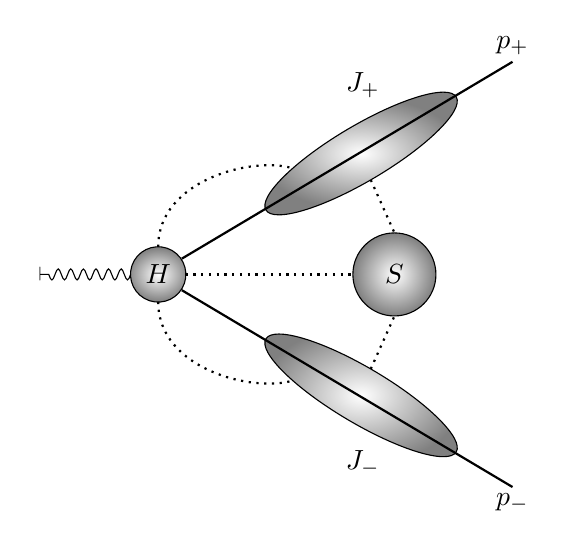
\begin{tikzpicture}
\shadedraw[inner color=white,outer color=gray,draw=black,rotate=30.7]  (3,0.005) ellipse (40pt and 10pt);
\shadedraw[inner color=white,outer color=gray,draw=black,rotate=-30.7]  (3,-0.005) ellipse (40pt and 10pt);
\shadedraw[inner color=white,outer color=gray,draw=black,rotate=-30]  (0,0) ellipse (10pt and 10pt);
\shadedraw[inner color=white,outer color=gray,draw=black]  (3,0) ellipse (15pt and 15pt);
\draw [thick](0.3,-0.2) -- (4.5,-2.7);
\draw [thick](0.3,0.2) -- (4.5,+2.7);
\draw (4.5,+2.9) node {$p_+$};
\draw (4.5,-2.9) node {$p_-$};
\draw (2.6,-2.4) node {$J_{-}$};
\draw (2.6,2.4) node {$J_{+}$};
\draw (0,0) node {$H$};
\draw (3,0) node {$S$};
\draw [decoration={aspect=0, segment length=1.6mm, amplitude=0.7mm,coil},decorate] (-0.35,0)   -- (-1.5,0)node {\tiny$|$};

 \draw [thick, dotted] (0,0.35) .. controls (0,1.2) and (1.2,1.5) .. (1.7,1.35);
  \draw [thick, dotted] (0,-0.35) .. controls (0,-1.2) and (1.2,-1.5) .. (1.7,-1.35);
 \draw [thick, dotted] (0.35,0) -- (2.47,0);
 \draw [thick, dotted] (2.7,-1.2) -- (3,-0.53);
  \draw [thick, dotted] (2.7,1.2) -- (3,0.53);

\end{tikzpicture}
\caption{Representation of the hard $(H)$, the soft $(S)$, and jet $J_{(\pm)}$ pinch surfaces for the quark electromagnetic vertex at all orders before power counting. The dotted lines represent all the possible lines (fermionic or gluonic) connecting different pinch surfaces. }\label{pinch}
\end{figure}

This reduced diagram corresponds to physical processes in which the photon decays into two jets $J_+$ and $J_-$ each with the total momenta, $p_1$ and $p_2$, as the two final state particles. Between these two jets the only interaction is via zero-momentum soft particles, labeled $S$. This is due to the fact that since, once the jets are formed, they travel in different directions at the speed of light and hence no finite momentum transfer can occur between the two. Higher order off-shell, short-distance contributions coming from shrunk lines are encoded in the subdiagram $H$. The full derivation of this characterization of general pinch surfaces to all orders in perturbation theory is presented in \cite{Sterman1}. The term pinch surface is introduced to illustrate the fact that the singularity configurations constrain loop momenta, defining a hypersurface in the $(\{\alpha\},\{k\})$ space where the singularity is pinched and hence is unavoidable. \par
The next step towards the factorization of the $qq\gamma$ amplitude is to power-count (this amounts to just counting the power of the so called normal variables, i.e. the ones where their vanishing defines the pinch surface, in the numerator and in the denominator of the integrand) and find the most divergent solutions to the Landau equations. In \cite{Sterman1} it is proven that in any covariant gauge, the divergencies are logarithmic at worst and the general pinch surface is of the form presented in Fig. \ref{pinch2} in $d=4$ dimensions. Where the jet functions $J_\pm$ are only connected to the hard function $H$ through one fermion line and longitudinally polarized gluons, the jets are connected to each other through longitudinally polarized gluons connected to the soft function $S$ \cite{Collins}. In all physical gauges the divergencies are also logarithmic at worst and furthermore no lines except for the fermionic lines connect $H$ to the jets $J_\pm$ \cite{Stermannotes}.
\begin{figure}[ht!]
\centering
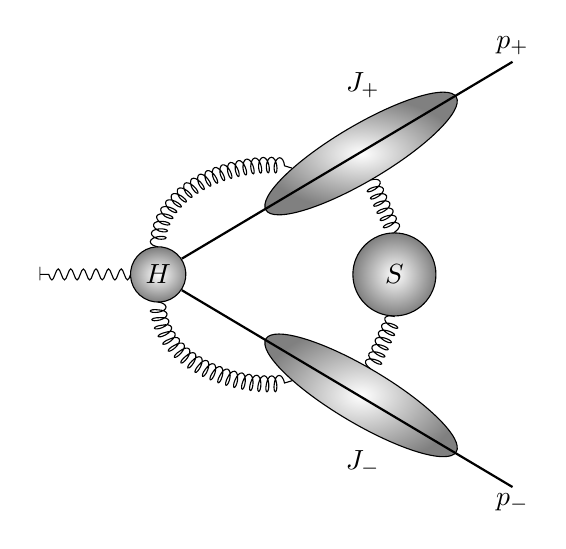
\begin{tikzpicture}
\shadedraw[inner color=white,outer color=gray,draw=black,rotate=30.7]  (3,0.005) ellipse (40pt and 10pt);
\shadedraw[inner color=white,outer color=gray,draw=black,rotate=-30.7]  (3,-0.005) ellipse (40pt and 10pt);
\shadedraw[inner color=white,outer color=gray,draw=black,rotate=-30]  (0,0) ellipse (10pt and 10pt);
\shadedraw[inner color=white,outer color=gray,draw=black]  (3,0) ellipse (15pt and 15pt);
\draw [thick](0.3,-0.2) -- (4.5,-2.7);
\draw [thick](0.3,0.2) -- (4.5,+2.7);
\draw (4.5,+2.9) node {$p_+$};
\draw (4.5,-2.9) node {$p_-$};
\draw (2.6,-2.4) node {$J_{-}$};
\draw (2.6,2.4) node {$J_{+}$};
\draw (0,0) node {$H$};
\draw (3,0) node {$S$};
\draw [decoration={aspect=0, segment length=1.6mm, amplitude=0.7mm,coil},decorate] (-0.35,0)   -- (-1.5,0)node {\tiny$|$};
 \draw [decoration={aspect=0.4, segment length=1mm, amplitude=1mm,coil},decorate] (0,0.35) .. controls (0,1.2) and (1.2,1.5) .. (1.7,1.35);
  \draw [decoration={aspect=0.4, segment length=1mm, amplitude=1mm,coil},decorate] (0,-0.35) .. controls (0,-1.2) and (1.2,-1.5) .. (1.7,-1.35);
% \draw [decoration={aspect=0.4, segment length=1mm, amplitude=1mm,coil},decorate] (0.35,0) -- (2.47,0);
 \draw [decoration={aspect=0.4, segment length=1mm, amplitude=1mm,coil},decorate] (2.7,-1.2) -- (3,-0.53);
  \draw [decoration={aspect=0.4, segment length=1mm, amplitude=1mm,coil},decorate] (2.7,1.2) -- (3,0.53);
%\draw [decoration={aspect=0.4, segment length=1mm, amplitude=1mm,coil},decorate] (4.5,+2.7) .. controls (4.7,2.) and (3.7,0.53) .. (3.3,0.42);
%\draw [decoration={aspect=0.4, segment length=1mm, amplitude=1mm,coil},decorate] (4.5,-2.7) .. controls (4.7,-2.) and (3.7,-0.53) .. (3.3,-0.42);
\end{tikzpicture}
\caption{General pinch surface corresponding to logarithmic divergences. Only gluons connecting the hard and soft to the jet surfaces can be present to give this divergence.}\label{pinch2}
\end{figure}

Our goal now is to factorize this general pinch surface into contributions where in each of the regions ($H$, $J_\pm$ and $S$) the loop momenta is not restricted anymore in a gauge independent way. This is performed through the introduction of the so called Wilson lines, which are related with the parallel transport in fibre bundles and the uniqueness of the so called ``horizontal lift'' \cite{Nakahara} of a spacetime curve $\gamma(t)$ with $t\in[t_1,t_2]$ between the two points $y=\gamma(t_1)$ and $z=\gamma(t_2)$
\begin{equation}
\Phi(t_2,t_1)\equiv \mathcal{P} \Big\{\exp\Big(-ig\mu^{\epsilon}\int_{t_1}^{t_2}dt\frac{d\gamma^\mu}{dt} A_\mu(\gamma(t))\Big)\Big\}\label{Wilsonline}
\end{equation}
where the symbol $\mathcal{P}$ is the path ordering operator which orders the $A_\mu(\gamma(t))$ so that the ones with higher $t$ stand to the left (remember that the $A$'s are matrices). \par
The Wilson lines are introduced since they reproduce order by order the so called eikonal Feynman rule of soft gluon emissions. This is so because soft gluons only ``know'' about the color and the direction of the jet they attach to. For this reason we will regard their interaction as eikonal.\par
 How is this related to the Wilson line? Recall that internal lines in reduced diagrams are in free-flight so that their velocity $v^\mu$ is constant along their trajectory and we can hence write (\ref{Wilsonline}) for these particles as
\begin{equation}
\Phi_v(t_2,t_1)=\mathcal{P} \Big\{\exp\Big(-ig\mu^{\epsilon}\int_{t_1}^{t_2}dtv^\mu A_\mu(tv)\Big)\Big\}\;.
\end{equation}
Considering now $\Phi(\infty,0)$ and expressing $A^\mu(x)$ as the sum of its Fourier coefficients we get
\begin{equation}
\Phi_v(\infty,0)=\mathcal{P} \Big\{\exp\Big(-ig\mu^{\epsilon}\int_{0}^{\infty}dtv^\mu\int\frac{d^Dk}{(2\pi)^D}\tilde{A}_\mu(k)e^{i t k\cdot v}\Big)\Big\} \;.
\end{equation}
To carry out the integration in $t$ we will Wick rotate $k^0\to ik^0$ so that the contribution from $t=\infty$ vanishes. In this way, after going back to real energy, we obtain
\begin{align}
\Phi_v(\infty,0)=\exp\Big(g\mu^{\epsilon}\int\frac{d^Dk}{(2\pi)^D}\frac{v^\mu}{k\cdot v}\tilde{A}_\mu(k)\Big)\;.
\end{align}
Which reproduces order by order the eikonal soft gluon emission from a fermion line.\par
Thanks to the introduction of the Wilson lines, the so called eikonal identity (which represents the fact that at leading order in softness soft emissions factorize and are expressed in terms of independent emissions with eikonal vertices), and the use of Ward identities, it is possible to factorize the all order quark EM form factor \cite{Collins}. This will lead to express the general pinch surface in Fig. \ref{pinch2} in the factorized form in Fig. \ref{factorized}.
Each pinch region we have identified above has its momentum variables restricted to a region in the phase space: in the soft and jet subdiagrams all the lines are soft and collinear respectively. Hence, the functions we want to define that encode the singularities in each subdiagram will also have to have their momenta restricted. This fact complicates a lot the factorization and this is why we will seek a formula in which line momenta are not restricted.\par
Let us begin defining the soft function as
\begin{equation}
\mathcal{S}(\beta_1\cdot \beta_2,\alpha_s(\mu^2),\epsilon)\equiv\bra{0} \Phi_{\beta_1}(\infty,0) \Phi_{\beta_2}(\infty,0)\ket{0}\;,\label{softf}
\end{equation}
where $\beta_+$ and $\beta_-$ are proportional to the jet momenta $p_+$ and $p_-$ respectively, $\mu^2$ is a renormalization scale and $\epsilon$ the dimensional regulator. We define now each jet leg as
\begin{equation}
J_\pm\Big(\frac{(p_\pm\cdot n_\pm)^2}{n_\pm^2\mu^2},\alpha_s(\mu^2),\epsilon\Big)u(p_\pm)=\frac{\bra{0} \Phi_{n_\pm}(\infty,0) \psi(0)\ket{p_\pm}}{\bra{0} \Phi_{n_
\pm}(\infty,0)\ket{0}}\,,\label{JET}
\end{equation}
where $\psi$ is the fermion field operator and $n_i$ is the direction of the Wilson line. To avoid spurious collinear singularities it is customary to choose $n_i^2\neq 0$. We introduce the denominator to cancel graphs with eikonal self interactions.\par
Now we need to take into account the overlap of the soft and collinear regions to avoid double counting. The overlapping can be seen as a jet function whose collinear gluons become soft or a soft function whose gluons become collinear. In either case, it can be described by the \textit{eikonal jet function} defined as
\begin{equation}
\mathcal{J}_i\Big(\frac{(\beta_i\cdot n_i)^2}{n_i^2\mu^2},\alpha_s(\mu^2),\epsilon\Big)\equiv\bra{0} \Phi_{n_i}(\infty,0) \Phi_{\beta_i}(\infty,0)\ket{0}\,.
\end{equation}
Defining the hard function $\mathcal{H}$ as the result of dividing the form factor $\Gamma$ by $\mathcal{S}\prod_i(J_i/\mathcal{J}_i)$, we can finally write the formula for the factorized form factor
\begin{align}
\Gamma\Big(\frac{\mu^2}{Q^2},\alpha_s(\mu^2),\epsilon\Big)&=\mathcal{H}	\Big(\frac{\mu^2}{Q^2},\alpha_s(\mu^2),\epsilon\Big)\mathcal{S}(\beta_1\cdot \beta_2,\alpha_s(\mu^2),\epsilon)\times\nonumber\\ &\times \prod_{i=\pm}\frac{J_i\Big(\frac{(p_i\cdot n_i)^2}{n_i^2\mu^2},\alpha_s(\mu^2),\epsilon\Big)}{\mathcal{J}_i\Big(\frac{(\beta_i\cdot n_i)^2}{n_i^2\mu^2},\alpha_s(\mu^2),\epsilon\Big)}\;.\label{factorization}
\end{align}
Here it is implied that, since the soft and jet functions present in (\ref{factorization}) can generate new UV divergences, UV counterterms are introduced to cancel UV divergences present in the soft and jet functions.  Note that these functions depend only on general properties of the external particles like spin, charge or color, and collect all soft and collinear divergences. This dependence and some issues concerning the so called \textit{cusp anomaly} of is studied in detail in \cite{DGM}. %can be shown as a consequence of the homogeneity with respect to the vectors $n^\mu$ by dimensional analysis involving $n^2\neq0$ \cite{Bonoc}. This fact cannot be said for $\beta^\mu$ since $\beta^2=0$ and it leads to the so called \textit{cusp anomaly} which happens to cancel.
The factorization formula (\ref{factorization}) can be extended to more generic amplitudes. In cases with more legs, the color dependence of the amplitude is non-trivial but remains treatable. However, the presence of the so called Glauber gluons might spoil factorization. This is still an open topic of research (see for example \cite{CFR}-\cite{FSS} for more recent and refined results).

\begin{figure}[ht!]
\centering
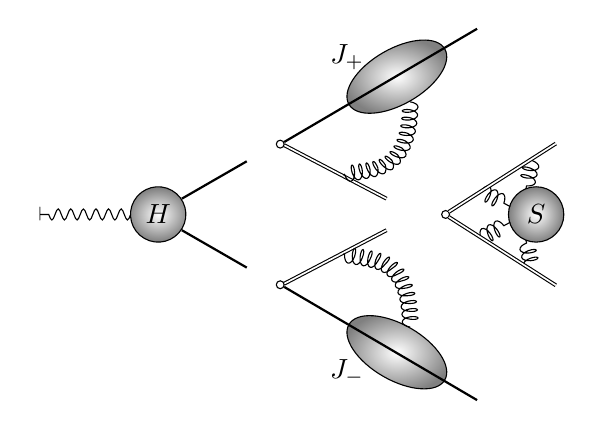
\begin{tikzpicture}

\shadedraw[inner color=white,outer color=gray,draw=black,rotate=30]  (3.5,-0.) ellipse (20pt and 10pt);

\shadedraw[inner color=white,outer color=gray,draw=black,rotate=-30]  (3.5,-0.) ellipse (20pt and 10pt);
\shadedraw[inner color=white,outer color=gray,draw=black,rotate=-30]  (0,0) ellipse (10pt and 10pt);
\shadedraw[inner color=white,outer color=gray,draw=black,rotate=0]  (4.8,0) ellipse (10pt and 10pt);
\draw [thick](0.3,-0.2) -- (1.125,-0.675);
\draw [thick](0.3,0.2) -- (1.125,+0.675);

\draw [thick](1.6,-0.92) -- (4.05,-2.358);
\draw [thick](1.6,0.92) -- (4.05,2.358);
\draw [double](1.6,-0.88) -- (2.9,-0.2);
\draw [double](1.6,0.88) -- (2.9,0.2);
\draw (0,0) node {$H$};
\draw (4.8,0) node {$S$};
 \draw (1.5,-0.893) arc [start angle=180, end angle=-180, radius=0.05cm];
  \draw (1.5,0.893) arc [start angle=180, end angle=-180, radius=0.05cm];
\draw (2.4,-2) node {$J_-$};
\draw (2.4,2) node {$J_+$};
\draw [decoration={aspect=0, segment length=1.6mm, amplitude=0.7mm,coil},decorate] (-0.35,0)   -- (-1.5,0)node {\tiny$|$};


\draw [decoration={aspect=0.4, segment length=1mm, amplitude=1mm,coil},decorate] (4.1,0.3)   -- (4.47,0.1);
\draw [decoration={aspect=0.4, segment length=1mm, amplitude=1mm,coil},decorate] (4.1,-0.3)   -- (4.47,-0.1);
\draw [decoration={aspect=0.4, segment length=1mm, amplitude=1mm,coil},decorate] (4.75,-0.685)   -- (4.67,-0.325);
\draw [decoration={aspect=0.4, segment length=1mm, amplitude=1mm,coil},decorate] (4.75,0.685)   -- (4.67,0.325);

 \draw (3.6,0) arc [start angle=180, end angle=-180, radius=0.05cm];
 \draw [double](3.69,0.032) -- (5.05,0.9);
  \draw [double](3.69,-0.032) -- (5.05,-0.9);
%\draw [decoration={aspect=0.4, segment length=1mm, amplitude=1mm,coil},decorate] (0.35,0) -- (2.47,0);

\draw [decoration={aspect=0.4, segment length=1mm, amplitude=1mm,coil},decorate]  (3.2,-1.43) .. controls (3.2,-0.5) and (2.7,-0.6) .. (2.35,-0.5);
\draw [decoration={aspect=0.4, segment length=1mm, amplitude=1mm,coil},decorate]  (3.2,1.43) .. controls (3.2,0.5) and (2.7,0.6) .. (2.35,0.5);
%\draw [decoration={aspect=0.4, segment length=1mm, amplitude=1mm,coil},decorate] (4.5,-2.7) .. controls (4.7,-2.) and (3.7,-0.53) .. (3.3,-0.42);
\end{tikzpicture}
\caption{Factorized quark EM form factor corresponding to equation (\ref{factorization}).}\label{factorized}
\end{figure}

\subsection{Coordinate-space factorization}
The momentum-space results presented above were extensively studied from the early 80's to the present day, however, the coordinate-space analogue results appeared only recently thanks to O. Erdogan's work \cite{ErdoganCS}. Here Erdogan presents a precise derivation of the factorization formulas for the quark EM form factor using the same steps as presented above. \par
 First the unavoidable singularities of coordinate-space Feynman graphs,
\begin{equation}
I(\{x_i^\mu\})=\prod_{\substack{\text{vertices}\\k}}\int d^Dy_k\prod_{\substack{\text{lines}\\j}}\frac{F(\{x_i\},\{y_k\})}{[z_j^2+i\eta]^{p_j}}\;,\label{fefo}
\end{equation}
 are identified using again the Coleman-Norton interpretation (here the $\{y_k^\mu\}$ are the position of internal vertices and $\{x_i^\mu\}$ the positions of external points. $F(\{x_i\},\{y_k\})$ is a numerator factor containing all color factors, constant and numerator factors, and $p_j$ depends if the line is scalar fermionic or bosonic):\par
 
For a general massless diagram, the pinched vanishing of the denominator defines the Landau equations in coordinate-space
\begin{empheq}[left=\empheqlbrace]{align}
\sum_{\substack{\text{lines } j\\ \text{at vertex } k}}\alpha_jz_j^\mu\epsilon_{kj}=0 &\;\;\;\;\text{and} \nonumber\\
  \alpha_j\,z^2_j=0 & \;\;,\label{kulete}
\end{empheq}
where $z_j^\mu$ denotes the argument of the denominator in propagator of line $j$. It is of course intended that these equations must be satisfied together with the vanishing of the overall denominator obtained after Feynman parametrization. To connect with the Coleman-Norton picture, identify the product $\alpha_j z_j^\mu$ with a momentum vector $l^\mu\equiv \lambda\alpha_j z^\mu_j$ and $\lambda\alpha_j\equiv l_j^0/z^0_j$. Note that in the coordinate-space picture the Feynman parameters are interpreted in the inverse way as in the momentum-space picture. This means that the soft singularities will have $\alpha_j=0$ and $\lambda$ can be set to one. For a hard singularity, i.e. $z^0_j=|\vec{z}_j|\to0$ (since $\alpha_j\neq0$) the $\lambda$ parameter helps $\alpha$ to remain finite and to have a non-zero momentum even if $z^\mu\to0$.
In this way we can see that each pinch singularity corresponds to massless particles propagating finite distance freely on the lightcone between vertices with their momenta satisfying momentum conservation at each vertex. On the other hand off-shell particles have zero displacement in divergent configurations. Solutions to the Landau equations not satisfying these conditions can be ruled out \cite{ErdoganCS}. \par
After identifying the pinch surfaces for the $\gamma q q$ vertex one can easily recognize the same surfaces as in the momentum pinture: two jets, one soft and one hard surface. Using the power-counting techniques it is possible to see that the singularities of the vertex at logarithmic at worst in $d=4$ dimensions and they correspond to the coordinate-space analogue of Fig. \ref{pinch2}, where only gluons connect the hard and soft with jet surfaces respectively \cite{ErdoganCS}. \par
Finally, after using the so called hard-collinear and soft-collinear approximations it is possible to see that the jets are connected to the soft and hard surfaced only by longitudinally polarized gluons (also known as scalar gluons). Due to this fact, Ward identities are used to factorize the vertex function as in Fig. \ref{factorized} \cite{ErdoganCS}.\par
Now we will turn to compute some contributions to the Jet function in coordinate-space. To be able to compare our results we present here the results from momentum-space calculations: \par
For the jet function at one loop we will have the contributions from a self energy correction $J_p^{(1)}$ of the quark line and a gluon exchange vertex correction $J_V^{(1)}$ between the Wilson and the fermion line. All these contributions including the UV counterterms are plotted in Fig. \ref{jetff}. The eikonal self interaction graphs do not appear due to the denominator in equation (\ref{JET}).
\begin{figure}[ht!]
\centering
\begin{tikzpicture}
\begin{feynman}
\vertex (a);
\vertex [right=2 cm of a] (b);
\vertex [right=1.6 cm of a] (b3);
\vertex [right=0.4 cm of a] (b4);
\vertex [below right=0.06 cm of b] (bs);
\vertex [right=0.01 cm of bs] (bss);
\vertex [below=1.4 cm of bss] (b1);






\diagram* {
(b)-- [fermion](a)
(b3)-- [gluon,half left,looseness=1.7](b4)
(b1)--[double] (bss)

};\draw (b) arc [start angle=180, end angle=-180, radius=0.05cm];
\end{feynman}
\end{tikzpicture}\;\;\;\;\;\;\;\;\;\;
\begin{tikzpicture}
\begin{feynman}
\vertex (a);
\vertex [right=2 cm of a] (b);
\vertex [right=1.6 cm of a] (b3);
\vertex [right=0.5 cm of a] (b4);
\vertex [below right=0.06 cm of b] (bs);
\vertex [right=0.01 cm of bs] (bss);
\vertex [below=1.4 cm of bss] (b1);
\vertex [below=0.9 cm of bss] (b12);






\diagram* {
(b)-- (a)
(b)-- [fermion](b4)
(b12)-- [gluon,half left,looseness=0.8](b4)
(b1)--[double] (bss)

};\draw (b) arc [start angle=180, end angle=-180, radius=0.05cm];
\end{feynman}
\end{tikzpicture}\\
$\;$\\
\begin{tikzpicture}
\begin{feynman}
\vertex (a);
\vertex [left=1cm of a] (ba1);
\vertex [right=2 cm of ba1] (b);
\vertex [right=1.6 cm of ba1] (b3);
\vertex [right=0.4 cm of ba1] (b4);
\vertex [below right=0.06 cm of b] (bs);
\vertex [right=0.01 cm of bs] (bss);
\vertex [below=1.4 cm of bss] (b1);







\diagram* {
a [dot];
(b)-- (a)--(ba1)
(b1)--[double] (bss)

};\draw (b) arc [start angle=180, end angle=-180, radius=0.05cm];
\end{feynman}
\end{tikzpicture}\;\;\;\;\;\;\;\;\;\;\;
\begin{tikzpicture}
\begin{feynman}
\vertex (a);
\vertex [left=2 cm of a] (b);
\vertex [right=1.6 cm of b] (b3);
\vertex [right=0.4 cm of b] (b4);
\vertex [below=0.07 cm of a] (bs);
\vertex [right=0.0 cm of bs] (bss);
\vertex [below=1.38 cm of bss] (b1);






\diagram* {
a [dot];
(a)-- [fermion](b)
(b1)--[double] (bss)

};
\end{feynman}
\end{tikzpicture}
\caption{Diagrams contributing to the first-order momentum-space jet function. The solid dots represent UV counterterms.}\label{jetff}
\end{figure}

The first diagram in Fig. \ref{jetff} vanishes in dimensional regularization since it is scaleless  (remember the external momentum is lightlike $p^2=0$) and there is no available quantity with non-zero mass dimension. This comes from a cancellation of UV and IR poles. Therefore, after introducing the UV counterterm we will obtain that $J_p^{(1)}=1/\epsilon$. The vertex correction in the second diagram in Fig. \ref{jetff} amounts to
\begin{align}
J_V^{(1)}&=8\pi i\mu^{2\epsilon}\times\nonumber\\ 
&\times\int\frac{d^Dk}{(2\pi)^D}\frac{1}{(k^2-i\eta)(k^2-2p\cdot k-i\eta)(2n\cdot k-i\eta)}\,,
\end{align}
which in the $\overline{\text{MS}}$ scheme and after substraction of the UV pole by adding the counterterm in the fourth diagram in Fig. \ref{jetff},
 results in \cite{Bonoc},
\begin{equation}
J_V^{(1)}=-\Big[\Big(\frac{n^24\pi\mu^2}{(2p\cdot n)^2}\Big)^\epsilon\Big(\frac{1}{\epsilon^2}+\frac{1}{\epsilon}+2+\frac{5\pi^2}{12}\Big)+\frac{2}{\epsilon}\Big]\;.\label{biblioroneo}
\end{equation}

 

 \subsubsection{One-loop Jet function in coordinate-space}
 Once we have seen that factorization of the vertex function in coordinate-space comes along pretty much as in the momentum-space picture, let us now compute the one-loop jet function in coordinate-space and see if, using the LSZ reduction formula, we can recover the results known in momentum-space. 
 \begin{figure}[ht!]
 \centering
 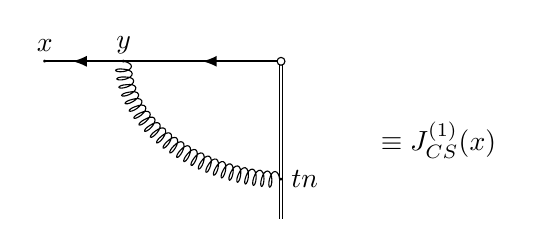
\begin{tikzpicture}[>=stealth]
 \draw [decoration={aspect=0.4, segment length=1mm, amplitude=1mm,coil},decorate] (1,0) .. controls (1,-0.9) and (2.1,-1.5) .. (3,-1.5);
 \draw[-latex,thick] (2.95,0)--(2,0);
  \draw[-latex,thick] (1,0)--(0.35,0);
    \draw [thick](0,0)--(0.55,0);
  \draw [thick](1,0)--(2.1,0);
   \draw (1,-0.01) node {$\cdot$};
      \draw (1,0.2) node {$y$};
          \draw (0,0.2) node {$x$};
          \draw (3.3,-1.5) node {$tn$};
          \draw (5,-1) node {$\equiv J^{(1)}_{CS}(x)$};
          
      \draw (0,-0.01) node {$\cdot$};
   \draw[double] (3,-0.05)--(3,-2);
   \draw (2.95,0) arc [start angle=180, end angle=-180, radius=0.05cm];
   \draw (3,-1.51) node {$\cdot$};
\end{tikzpicture}
\caption{Diagram representing the one-loop jet function (without UV conterterms) in coordinate-space.}\label{repera}
\end{figure}

Reading from Fig. \ref{repera} we have that, taking the Wilson line to be lightlike ($n^2=0$),
\begin{align}
J^{(1)}_{CS}&(x)=\frac{\Gamma(1-\epsilon)\Gamma^2(2-\epsilon)}{(2\pi^{2-\epsilon})^24\pi^{2-\epsilon}}\int d^D y \frac{-(\slashed{x}-\slashed{y})}{((x-y)^2+i\eta)^{2-\epsilon}}\times\nonumber\\&\times(-ig T^a\gamma_\mu)\frac{-\slashed{y}}{(y^2+i\eta)^{2-\epsilon}}\int_0^{+\infty}dt \frac{(-igT^a)n^\mu}{((y-tn)^2+i\eta)^{1-\epsilon}}\,.\label{tonaser}
\end{align}
We can introduce Feynman parameters in two steps combining firstly the second and third denominators in the integrands above and secondly the resulting denominator with the first one above to identify the different configurations giving rise to unavoidable divergences. We will also employ this Feynman parametrization to solve the whole integral. In this case, using the delta functions in the Feynman parameters, the Landau equations read 
\begin{align}
&\alpha_2(x-y)^2+(1-\alpha_2)\alpha_1 y^2+\nonumber\;\;\;\;\;\;\;\;\;\;\;\;\\
&\;\;\;\;\;\;\;\;\;\;\;\;\;\;\;\;\; +(1-\alpha_2)(1-\alpha_1)(y^2-2tn\cdot y)=0\,,\\
&\alpha_2(x-y)^\mu+(1-\alpha_2)\alpha_1 y^\mu+\nonumber\;\;\;\;\;\;\;\;\;\;\\
& \;\;\;\;\;\;\;\;\;\;\;\;\;\;\;\;\;+(1-\alpha_2)(1-\alpha_1)(y^\mu-tn^\mu)=0\;.
\end{align}
To study the case when the gluon line becomes soft we take $\alpha_1=1$. In this case we do not expect the gluon to change de direction of the external line since it carries no momentum. This is indeed the case because the solution to the Landau equations tells us that 
\begin{equation}
y^\mu=\frac{\alpha_2}{2\alpha_2-1} x^\mu\,,\label{lanroneador}
\end{equation}
and that $x$ and $y$ must lie in the lightcone for $\alpha_2\neq 0,1$.
For the end-point singularities in the $\alpha$ parameters we see that for $\alpha_2=1$ the vertex $y$ migrates to the external point. This makes sense since the fermion line from $0$ to $y$ will be carrying all the momentum while the fermion line from $y$ to $x$ shrinks. Taking $\alpha_2=0$ means that the $y$ vertex migrates to the origin, signaling that we are dealing with an UV divergence. However in both cases there is not restriction to $y$ or $x$ to lie on the lightcone.
\par
For the case when $\alpha_1=0$, so that the gluon is not soft, the Landau equations tell us that
\begin{equation}
y^\mu=\frac{(1-\alpha_2)tn^\mu-\alpha_2 x^\mu}{(1-2\alpha_2)}\;.
\end{equation}
As we will see below, the only contribution to this amplitude will come when $t=0$ so that we will have a collinear pinch surface with the vertex $y$ obeying (\ref{lanroneador}) but this time the gluon emerges from the Wilson line cusp (the origin), making the gluon collinear. Both the fermion external line and gluon lines are lightlike for $\alpha_2\neq0,1$. Again if $\alpha_2=1$ the internal vertex $y$ migrates to the external point $x$ and if $\alpha_2=0$ we will have that $y^\mu=tn^\mu$ signaling again a UV divergence for $t=0$.
\par
To carry out the whole integral we will introduce Feynmann parameters in two steps as above, first combining the second and third denominators and then the resulting denominator with the first one in (\ref{tonaser}). In this way
\begin{align}
&J^{(1)}_{CS}(x)=-g^2 C_F\frac{\Gamma(1-\epsilon)\Gamma^2(2-\epsilon)}{16\pi^{6-3\epsilon}}\frac{\Gamma(5-3\epsilon)}{\Gamma^2(2-\epsilon)\Gamma(1-\epsilon)}\times\nonumber\\
&\times\int d^D y\int_0^{+\infty}dt\int_0^1 d\alpha_1d\alpha_2\nonumber\times\\
&\frac{(\slashed{x}\slashed{n}\slashed{y}-\slashed{y}\slashed{n}\slashed{y})\alpha_1^{1-\epsilon}(1-\alpha_1)^{-\epsilon}\alpha_2^{1-\epsilon}(1-\alpha_2)^{2-2\epsilon}}{(y^2-2y\cdot(\alpha_2 x+(1-\alpha_1)(1-\alpha_2)tn)+\alpha_2 x^2+i\eta)^{5-3\epsilon}}\;.
\end{align}
Now we shift the integration variable $y\to y-(\alpha_2 x+(1-\alpha_1)(1-\alpha_2)tn)$ and, by parity, drop odd powers of the new $y$ in the numerator. This yields
\begin{align}
&J^{(1)}_{CS}(x)=-g^2 C_F\frac{\Gamma(5-3\epsilon)}{16\pi^{6-3\epsilon}}\int d^D y\int_0^{+\infty}dt\int_0^1 d\alpha_1d\alpha_2\times\nonumber\\
&\times\frac{(\alpha_2(1-\alpha_2)\slashed{x}\slashed{n}\slashed{x}-\slashed{y}\slashed{n}\slashed{y})\alpha_1^{1-\epsilon}(1-\alpha_1)^{-\epsilon}\alpha_2^{1-\epsilon}(1-\alpha_2)^{2-2\epsilon}}{(y^2+\alpha_2(1-\alpha_2) x^2-2(1-\alpha_1)(\alpha_2-\alpha_2^2)tn\cdot x+i\eta)^{5-3\epsilon}}\;.
\end{align}
It is possible (taking $y$ to be non-collinear with $n$ so that $n\cdot y\neq0$, which does not affect the integral since it is a measure zero region that we are avoiding in the integration volume) at this point to carry out the integration in $t$, producing
\begin{align}
&J^{(1)}_{CS}(x)=g^2 C_F\frac{\Gamma(5-3\epsilon)}{16\pi^{6-3\epsilon}}\int d^D y\int_0^1 d\alpha_1d\alpha_2\nonumber\times\\
&\frac{(\alpha_2(1-\alpha_2)\slashed{x}\slashed{n}\slashed{x}-\slashed{y}\slashed{n}\slashed{y})\alpha_1^{1-\epsilon}(1-\alpha_1)^{-1-\epsilon}\alpha_2^{-\epsilon}(1-\alpha_2)^{1-2\epsilon}}{(4-3\epsilon) 2n\cdot x(y^2+\alpha_2(1-\alpha_2) x^2+i\eta)^{4-3\epsilon}}\;.
\end{align}
Using standard Dimensional Regularization formulas we carry out the integral in $y$ and identify the Euler Beta functions in the Feynmann parameters integrations to get
\begin{align}
J^{(1)}_{CS}&(x)=\frac{-i\pi^{\frac{D}{2}}g^2 C_F(x^2)^{2\epsilon-2}}{(2x\cdot n) 16\pi^{6-3\epsilon}}\frac{\Gamma(1-2\epsilon)\Gamma(2-\epsilon)\Gamma(-\epsilon)}{\Gamma(2-2\epsilon)}\times\nonumber\\
&\times\Big(\frac{\Gamma(1+\epsilon)}{\Gamma(2+\epsilon)}+\frac{\Gamma(\epsilon)}{\Gamma(2+\epsilon)}\Big)\Big(2x\cdot n \slashed{x}(1-2\epsilon)+\epsilon\slashed n x^2\Big)\;.
\end{align}
Where in the Euler Beta function for the parameter $\alpha_2$ we used the trick of multiplying by $\alpha_2+(1-\alpha_2)$ to separate the finite part when $\alpha_2=1$ (corresponding to the first Gamma function fraction in the second line), from the UV divergence arising when $\alpha_2=0$ (corresponding to the second Gamma function fraction in the second line), so that the denominators $y^2$ and $(y-nt)^2$ are active in producing the UV divergence when $y^\mu,t\to0$ (this is also due to the analysis we have made above of the Landau equations where $\alpha_2=0$ signaled a UV divergence). This means that the renormalized one-loop jet function, $J^{(1)}_{CS\,r}$, amounts to 
\begin{align}
J^{(1)}_{CS\,r}(x)=&-i\pi^{\frac{D}{2}}\frac{g^2 C_F(x^2)^{2\epsilon-2}}{(2x\cdot n) 16\pi^{6-3\epsilon}}\frac{\Gamma(1-2\epsilon)\Gamma(2-\epsilon)\Gamma(-\epsilon)}{\Gamma(2-2\epsilon)}\nonumber\\
&\times\frac{\Gamma(1+\epsilon)}{\Gamma(2+\epsilon)}\Big(2x\cdot n \slashed{x}(1-2\epsilon)+\epsilon\slashed n x^2\Big)\;.
\end{align}
This expression, expanded to zeroth order in $\epsilon$, has the behavior
\begin{align}
J^{(1)}_{CSr}&(x)=\frac{i \alpha_s C_F}{4\pi}\frac{-\slashed x}{2\pi^2(x^2+i\eta)^2}\times \nonumber\\
&\times\Big(-\frac{2}{\epsilon}+4(1- \gamma_E)-(\slashed x)^{-1}\frac{\slashed n x^2}{n\cdot x}\Big)+O(\epsilon)\;.
\end{align}
This is a very nice result since the most divergent part is proportional to a Fermion propagator $S(x)$ (one can think of this result as follows: the gluon merges collinearly with the fermion producing the divergence times the propagator) and this will allow us to use the LSZ formula to get the momentum-space expression in a very simple manner. This formula relates the Jet function in momentum-space with the one in coordinate-space as
\begin{align}
J_{MS}(p)=-i\int {d^Dx} e^{-ip\cdot x} (-i\slashed\partial)J^{(1)}_{CSr}(x)\;,
\end{align}
By using the Dirac equation $\slashed\partial S(x)=i\delta^{(D)}(x)$ we find that the most divergent part of the jet function is
\begin{align}
\lim_{\epsilon\to0}J_{MS}(p)=\lim_{\epsilon\to0}\frac{\alpha_s C_F}{4\pi} \Big(-\frac{2}{\epsilon}\Big)\;.
\end{align}
So that we reproduce exactly the same pole structure as the renormalized one-loop gluon exchange vertex correction $J_V^{(1)}$ in (\ref{biblioroneo}) when $n^2=0$, disregarding the term containing $n^2$ (which would not have appear if in the calculation $n$ is taken lightlike from the beginning). \par 
However one could be doubtful of this $ad$ $hoc$ ``renormalization'', hence, we present hereby the full result of the jet function,
\begin{align}
J^{(1)}_{CS}(x)=&\frac{i \alpha_s C_F}{4\pi}\frac{-\slashed x}{2\pi^2(x^2+i\eta)^2}\times\nonumber\\
&\times\Big(-\frac{2}{\epsilon^2}+\frac{2(1-2\gamma_E)}{\epsilon}-(\slashed x)^{-1}\frac{\slashed n x^2}{n\cdot x}\frac{1}{\epsilon}\Big)+O(\epsilon^0)\;,
\end{align}
where the double pole expected in \cite{Bonoc} appears.
\subsection{One-loop jet function with internal gluon emission in coordinate-space}

Let us now compute the diagram in Fig. \ref{repera2} contributing to the one-loop radiated jet function in coordinate-space. We consider a lightlike Wilson line, i.e. $n^2=0$. 

\begin{figure}[ht!]
 \centering
 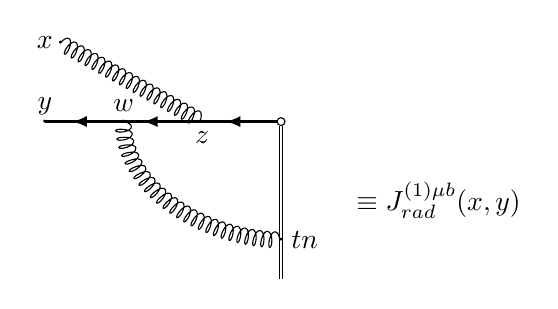
\begin{tikzpicture}[>=stealth]
 \draw [decoration={aspect=0.4, segment length=1mm, amplitude=1mm,coil},decorate] (1,0) .. controls (1,-0.9) and (2.1,-1.5) .. (3,-1.5);
  \draw [decoration={aspect=0.4, segment length=1mm, amplitude=1mm,coil},decorate] (.2,1) -- (2,0);
 \draw[-latex,thick] (2.95,0)--(2.3,0);
 \draw[-latex,thick] (2.6,0)--(1.25,0);
  \draw[-latex,thick] (1,0)--(0.35,0);
    \draw [thick](0,0)--(0.55,0);
  \draw [thick](1,0)--(2.1,0);
   \draw (1,-0.01) node {$\cdot$};
   \draw (1.98,-0.01) node {$\cdot$};
      \draw (.2,0.99) node {$\cdot$};
      \draw (1,0.2) node {$w$};
      \draw (2,-0.2) node {$z$};
      \draw (0,1) node {$x$};
          \draw (0,0.2) node {$y$};
          \draw (3.3,-1.5) node {$tn$};
          \draw (5,-1) node {$\equiv J^{(1)\mu b}_{rad}(x,y)$};
          
      \draw (0,-0.01) node {$\cdot$};
   \draw[double] (3,-0.05)--(3,-2);
   \draw (2.95,0) arc [start angle=180, end angle=-180, radius=0.05cm];
   \draw (3,-1.51) node {$\cdot$};
\end{tikzpicture}
\caption{Diagram representing the one-loop internal gluon emission from a jet.}\label{repera2}
\end{figure}

This diagram amounts to
\begin{align}
&J^{(1)\mu\,b}_{rad}(x,y)=(ig^3T^aT^bT^a)\Big(\frac{\Gamma(2-\epsilon)}{2\pi^{2-\epsilon}}\Big)^3\Big(\frac{\Gamma(1-\epsilon)}{4\pi^{2-\epsilon}}\Big)^2\times\nonumber\\
&\int d^Dzd^Dw \int_0^\infty d t \frac{-(\slashed y-\slashed w)}{((w-y)^2+i\eta)^{2-\epsilon}} \frac{-\slashed n(\slashed w-\slashed z)}{((w-z)^2+i\eta)^{2-\epsilon}}\times\nonumber\\
&\times \gamma^\mu\frac{-\slashed z}{(z^2+i\eta)^{2-\epsilon}}\frac{1}{((w-tn)^2+i\eta)^{1-\epsilon}}\frac{1}{((x-z)^2+i\eta)^{1-\epsilon}}\;.
\end{align}
The color structure above is easily computable, it gives $T^aT^bT^a=-T^b/2N$ for $SU(N)$. This factor is also computed for $SO(N)$, where is just $T^b/4$ (giving no suppression of the diagram for large number of colors), and for $Sp(N)$ where it amounts to $-T^b/4$.\par
As in the previous subsection we introduce Feynman parameters in two steps for combining the second, the third, and last denominators above such that
\begin{align}
&J^{(1)\mu\,b}_{rad}(x,y)=F^b\int d^Dw\int d^Dz\int_0^\infty dt \int_0^1d\alpha_1d\alpha_2\\
&\;\;\;\;\;\;\times\frac{(\alpha_1^{1-\epsilon}(1-\alpha_2)^{1-\epsilon}\alpha_2^{3-2\epsilon}(1-\alpha_1)^{-\epsilon})}{((w-y)^2+i\eta)^{2-\epsilon}((w-tn)^2+i\eta)^{1-\epsilon}}\times\nonumber\\
&\frac{(\slashed y-\slashed w)\slashed n \slashed z\gamma^\mu \slashed z-(\slashed n w^2+\slashed y \slashed n \slashed w)\gamma^\mu \slashed z}{(z^2-2z\cdot (\alpha_1\alpha_2 w+(1-\alpha_2)x)+\alpha_1\alpha_2 w^2+(1-\alpha_2)x^2)^{5-3\epsilon}}\;,
\end{align}
where $F^b$ encodes the color structure and numerical factors. Now, to compute the integral in $z$, we shift it as $z\to z-(\alpha_1\alpha_2 w+(1-\alpha_2)x)$ and then drop odd powers of $z$ in the numerator due to parity. This integration results in
\begin{align}
J^{(1)\mu\,b}_{rad}(x,y)&=F'^b\int d^Dw\int_0^\infty dt \int_0^1d\alpha_1d\alpha_2\nonumber\\
&\times\frac{(\alpha_1^{1-\epsilon}(1-\alpha_1)^{1-\epsilon}\alpha_2^{3-2\epsilon}(1-\alpha_1)^{-\epsilon})}{((w-y)^2+i\eta)^{2-\epsilon}((w-tn)^2+i\eta)^{1-\epsilon}}\times\nonumber\\
&\times \Big((\slashed w-\slashed y)\slashed n \gamma^\mu (m^2)+K^\mu\Big)(m^2)^{2\epsilon-3}\;,
\end{align}
where $m^2=\alpha_1\alpha_2(1-\alpha_1\alpha_2)w^2+\alpha_2(1-\alpha_2)x^2-2\alpha_1\alpha_2(1-\alpha_2)  x\cdot w$ and $K^\mu=(\slashed y-\slashed w) \slashed n (\alpha_1\alpha_2 \slashed w+(1-\alpha_2)\slashed x)\gamma^\mu(\alpha_1\alpha_2 \slashed w+(1-\alpha_2)\slashed x)-(2
w^2\slashed n+\slashed y\slashed n \slashed w)\gamma^\mu(\alpha_1\alpha_2 \slashed w+(1-\alpha_2)\slashed x)$. Next we combine the second denominator above with the last one again with Feynman parameters and then compute the integral in $t$ assuming we are not integrating $w$ in the region where $w\cdot n=0$. From this integration we will obtain a denominator factor and a $2x\cdot w$. We will combine these with the propagator denominator that was left in two steps of Feynman parametrization, which gives
\begin{align}
&J^{(1)\mu\,b}_{rad}(x,y)=F''^b\int d^Dw \int_0^1d\alpha_1...d\alpha_5\nonumber\\
&\times{\alpha_1^{1-\epsilon}(1-\alpha_1)^{1-\epsilon}\alpha_2^{3-2\epsilon}(1-\alpha_2)^{-\epsilon}\alpha_3^{-1-\epsilon}(1-\alpha_3)^{2-2\epsilon}}\times\nonumber\\
&\times \frac{\alpha_4^{2-3\epsilon}(1-\alpha_4)^{1-\epsilon}\alpha_5^{4-4\epsilon}}{(\alpha w^2+2w\cdot (\square)+\kappa^2)^{6-4\epsilon}}\Big((\slashed w-\slashed y)\slashed n \gamma^\mu (m^2)+K^\mu\Big)\;.
\end{align}
Here $\alpha=\alpha_3\alpha_4\alpha_5+\alpha_5(1-\alpha_3)\alpha_1\alpha_2(1-\alpha_1\alpha_2)+\alpha_5(1-\alpha_4)$, $(\square)^\mu=(1-\alpha_5)n^\mu-\alpha_1\alpha_2(1-\alpha_2)x^\mu-\alpha_5(1-\alpha_4)y^\mu$, and $\kappa^2=\alpha_5(1-\alpha_3)\alpha_2(1-\alpha_2)x^2+\alpha_5(1-\alpha_4)y^2$. Finally we shift the integration variable as $w\to w\alpha^{\frac{1}{2}}+(\square)\alpha^{-\frac{1}{2}}$ and carry out the $w$ integration finding
\begin{align}
&J^{(1)\mu\,b}_{rad}(x,y)=\frac{ig^3\pi^{3\epsilon-6}T^b}{2^8N(3-3\epsilon)}\times\int_0^1d\alpha_1...d\alpha_5\alpha_1^{1-\epsilon}(1-\alpha_1)^{1-\epsilon}\nonumber\\
&\times\alpha_2^{3-2\epsilon}(1-\alpha_2)^{-\epsilon}\alpha_3^{-1-\epsilon}(1-\alpha_3)^{2-2\epsilon} \alpha_4^{2-3\epsilon}(1-\alpha_4)^{1-\epsilon}\times\nonumber\\
&\times\alpha_5^{4-4\epsilon}\Big(g^{\rho\sigma}A^\mu_{\rho\sigma}\Gamma(3-3\epsilon)(M^2)+B^\mu\Gamma(4-3\epsilon)\Big)(M^2)^{3\epsilon-4}\;,\label{HAHAHA}
\end{align}
for $SU(N)$.
The expressions for the $A_{\rho\nu}^\mu$, $B^\mu$, and $M^2$ factors are shown in Appendix A. This result is not very enlightening since I have not been able to untangle the $\alpha$ parameters integrals while the tensor part is rather cumbersome and long. I expect that a better parametrization of the integral may give nicer results.


\section{Time Ordered Perturbation Theory}
In this section we will first review the known results from momentum-space TOPT, which are in deep connection with the Coleman-Norton picture. To offer an alternate perspective and further insights we will derive the coordinate-space counterpart to all orders in perturbation theory. 

\subsection{Momentum-space TOPT}

In quantum mechanics, transition amplitudes between unperturbed initial and final states represented by Green's functions are constructed from (virtual) unperturbed states through which the system passes during the transition. This picture is also present in QFT Feynman diagrams, even if it is not obvious, since we know that internal lines are usually off-shell.Thanks to the Coleman-Norton interpretation \cite{ColNor} (which helps finding unavoidable singularities in amplitudes), it is known that, in configurations giving rise to the IR leading contributions, the intermediate states traveling a noticeable distance are on-shell. Feynman integrals can be re-expressed in a way such that this connection becomes transparent.\par
   
        Any Green's function is a sum of all the covariant Feynman graphs contributing to the amplitude, this sum is equivalent to the sum of time ordered (TO) diagrams. These are topologically equivalent to covariant diagrams but with their vertices ordered in time. Hence, a covariant graph with $V$ vertices corresponds to up to $V!$ TO diagrams (we do not need to count permutation of vertices giving identical configurations [2]). TO graphs with external momenta $\{p\}$ are defined as
\begin{align}
\Gamma(\{p\})=&\prod_{loops\;i}\int\frac{d^3\vec{l}_i}{(2\pi)^3}\prod_{int.\;lines\;j}\frac{N(\{p\},\{l_i\})}{2\omega_j(\{l_i\},\{p\})}\times\nonumber\\
\times&\prod_{states\,a}\frac{1}{E_a-S_a+i\eta}\label{TOdiag}\,,
\end{align}
times a $-(2\pi)\delta(E_{in}-E_{out})$. Here the set of lines between the $a$th vertex and the $(a+1)$th vertex define the ``state'' $a$. $E_a$ is the ``energy of the state $a$'', i.e. the energy that has flowed into the diagram up to the $a$th vertex. $S_a$ is the ``on-shell'' energy of state $a$, which is the sum of of the mass-shell energies of each of the lines in $a$, $
S_a=\sum_{j\;\in \;a}\omega_j=\sum_{j\;\in\;a}\sqrt{\vec{k}_j^2+m_j^2}\;.$
The factor $N(\{p\},\{l_i\})$ represents numerator factors and $\{k_j\}$ are momenta in each internal line. \\

This general form of TO diagrams is proved carrying out the integrations in the time components of the loop momenta $\{l_i\}$. We see therefore that, in Feynman diagrams, energy is conserved at each vertex but having lines off the mass shell while in time-ordered perturbation theory all lines are on-shell but energy is not conserved at the vertices (of course the external energy flow is conserved). As an example let us see how the one-loop self energy scalar (cubic) Feynmann graph (with incoming (outgoing) momentum $p_0$ ($p'_0$) and loop momentum $k$) is expressed as a sum of two different time-ordering of the internal vertices. To see this fact and get an intuition of how eq. (1) is obtained we compute the energy integral of the loop momentum for the self-energy graph giving the integrand (to be integrated over space component of the loop momentum $k$)
\begin{align}
&I(p,p')=-(2\pi)\delta(p_0-p_0')\times\nonumber\\
&\times\frac{1}{2\omega2\omega'}\Big[\frac{1}{p_0-\omega-\omega'+i\eta}+\frac{1}{-p_0-\omega-\omega'+i\eta}\Big]\;,\label{fetonia}
\end{align}
where $\omega=\sqrt{\vec{k}^2+m^2}$ and $\omega'=\sqrt{\vec{k}'^2+m^2}=\sqrt{(\vec{k}-\vec{p}\,)^2+m^2}$.\par

\begin{figure}[ht!]
\centering
\begin{tikzpicture}
\begin{feynman}
\vertex (a);
\vertex [left=1.3 cm of a] (b);
\vertex [right=2 cm of a] (c);
\vertex [right=1.3 cm of c] (d);
\vertex [below right=1.3 cm of a] (bzz){};
\vertex [left=0.06 cm of bzz] (bz1z){(a)};




\diagram* {
(b)-- [momentum=$p_0$](a)
(a)--[half left, looseness=1.3] (c)
(a)--[half right, looseness=1.3] (c)
(c)-- [momentum=$p'_0$](d)
};
\end{feynman}
\end{tikzpicture}
\;\;\;\;\;\;\;
\begin{tikzpicture}
\begin{feynman}
\vertex (a);
\vertex [above left=0.095 cm of a] (b1);
\vertex [left=0.09 cm of b1] (b11);
\vertex [left=1.5 cm of b1] (b);
\vertex [below left=2 cm of a] (c);
\vertex [below right=0.095 cm of c] (c1);
\vertex [right=0.09 cm of c1] (c11);
\vertex [right=1.5 cm of c1] (d);
\vertex [below=1.8 cm of a] (bzz);
\vertex [left=0.4 cm of bzz] (bzz1){(b)};



\diagram* {
(b)--[momentum=$p_0$](b11)
(a)--[half left, looseness=0.7] (c)
(a)--[half right, looseness=0.7] (c)
(c11)--(d)
};
\end{feynman}
\end{tikzpicture}
\caption{TO diagrams whose sum corresponds to the one-loop self energy Feynman graph. The time ordering of internal vertices goes from left to right. The first case corresponds to an incoming particle with energy $p_0$ which decays into two virtual states with on-shell energies $\omega$ and $\omega'$ which recombine into the state with energy $p_0'$. The second case corresponds to a free particle with energy $p_0$ that annihilates with two out of three particles originating from the vacuum with energy $\omega$ and $\omega'$ with their total energy adding up to $-p_0'$. The third particle coming from the vacuum with momentum $p_0'$ travels freely to the final state.} \label{asddasdas}
\end{figure}
$\;$\\


This treatment offers a neat interpretation of the Feynman parameters $\alpha_j$  if one represents the TO diagram denominators in exponential form and performs a stationary phase approximation \cite{Stermannotes},
\begin{equation}
\sum_{a\;(j\;in\; a)}\Big(\frac{\tau_{a+1}-\tau_a}{\omega_j}\Big)=\lambda\,\alpha_j\;.
\end{equation}
With this result at hand it is easy now to interpret things in terms of the Coleman-Norton picture. An off-shell particle in line $j$ has $\alpha_j=0$, that is,  its flying time is really small or/and its spatial momentum is huge such that $\omega_j$ is very large. In collinear cases we will obtain a relationship between the $\omega$s of the jet particles. Finally, we see that for soft cases, $\omega$ goes to zero and we need the scale $\lambda$ to infinity to keep the flying time and $\alpha$ finite. \par
It is also possible to prove unitarity in momentum-space TOPT in a rather straightforward way, we present the original (although not new) proof using mathematical induction in Appendix B.

\subsection{Coordinate-space TOPT to all orders}

Now let us study TOPT in coordinate-space.  A general expression for an arbitrary connected massless scalar diagram with $E$ fixed external points and $L$ lines in four dimensional coordinate representation is
\begin{equation}
G_e(\{x_a\})=\frac{(-ig)^N}{(4\pi^2)^L}\int\prod_{\substack{\text{vertices}\\i=1}}^Nd^4y_i\prod_{\text{lines}\;j}^L\frac{1}{z_j^2(y_i,x_a)+i\eta}\;,\label{dadada44}
\end{equation}
where the $x_a$, $a=1,...,E$, denote the external points and the $y_i$ the internal vertices, and the vectors $z_j^\mu$, $j=1,...,L$, defined by
\begin{equation}
z_j^\mu=(\epsilon_{ji}y_i+\epsilon'_{ja}x_a)^\mu\;.
\end{equation}
The incidence matrix elements $\epsilon_{ji}$ take the value $+1$ $(-1)$ when $z_j$ is defined to end (begin) at vertex $i$, and zero otherwise, and similarly for $\epsilon'_{ja}$ in terms of external vertices $x_a$. Now we insert the identity in (\ref{dadada44}) as
\begin{align}
G_e(\{x_a\})=&\frac{(-ig)^N}{(4\pi^2)^L}\int\prod_{\substack{\text{vertices}\\i=1}}^Nd^4y_i\times\nonumber\\
&\times\prod_{\text{lines}\;j}^L\int dz^0_{j}\frac{\delta(z_{j}^0-\epsilon_{jk}y_k^0-\epsilon'_{jc}x^0_c)}{-{z_{j}^0}^2+{\vec{z}_j}^{\;2}+i\eta}\;,\label{dadada441}
\end{align}
where summation over $k=1,...,N$ and $c=1,...,E$ is intended. Next we re-express each delta function as an integral over an auxiliary variable with units of  energy, $E^0_j$,
\begin{align}
G_e(\{x_a\})=&\frac{(-ig)^N}{(4\pi^2)^L}\int\prod_{\substack{\text{vertices}\\i=1}}^Nd^4y_i\prod_{\text{lines}\;j}^L\times\nonumber\\
&\times\int_{-\infty}^{+\infty}dz_{j}^0\int_{-\infty}^{+\infty}\frac{dE^0_j}{2\pi}\frac{e^{iE^0_j(z_{j}^0-\epsilon_{jk}y^0_k-\epsilon'_{jc}x^0_c)}}{-{z_{j}^0}^2+{\vec{z}_j}^{\;2}+i\eta}\;,\label{dadada442}
\end{align}
and carrying out the integrations in $z^0_j$ we get
\begin{align}
&G_e(\{x_a\})=\frac{(-ig)^N i^L}{(4\pi^2)^L}\int\prod_{\substack{\text{vertices}\\i=1}}^Nd^4y_i\nonumber\prod_{\text{lines}\;j}\frac{1}{2|{\vec{z}_j|+i\eta}}\times\\
&\times\int_{-\infty}^{+\infty}{dE^0_j}\Big(\theta (E^0_j)e^{-iE_j^0(\epsilon_{jk}y^0_k+\epsilon'_{jc}x^0_c-|\vec{z}_j|-i\eta)}+\nonumber\\
&\;\;\;\;\;\;\;\;\;\;\;\;\;\;\;\;\;\;+\theta (-E^0_j)e^{-iE_j^0(\epsilon_{jk}y^0_k+
\epsilon'_{jc}x^0_c+|\vec{z}_j|+i\eta)}\Big)\;.\label{dadada443}
\end{align}
Finally, integrating over the time component of the internal vertices, $y^0_j$, we obtain
\begin{align}
&G_e(\{x_a\})=\frac{(-ig)^Ni^L(2\pi)^N}{(4\pi^2)^L}\int\Big(\prod_{\substack{\text{vertices}\\i=1}}^Nd^3y_i\Big)\prod_{\text{lines}\;j}^L\int_{-\infty}^{+\infty}{dE^0_j}\nonumber\\
&\times\frac{\theta(E_j^0)e^{-iE_j^0(\epsilon'_{jc}x^0_c-|\vec{z}_j|-i\eta)}+\theta(-E_j^0)e^{-iE_j^0(\epsilon'_{jc}x^0_c+|\vec{z}_j|+i\eta)}}{2|{\vec{z}_j}|+i\eta}\nonumber\\&\times\prod_{i=1}^N\delta\Big(\sum_{l=1}^LE_{l}^0\epsilon_{li}\Big)\;.\label{dadada444}
\end{align}
From this equation we can see that there is energy conservation at each vertex and that the $\theta$-functions produce the same result as in the study of the Largest Time Equation \cite{Veltman2}, where energy can flow forward or backwards in the time ordering. This is the main difference with the lightcone ordered perturbation theory where energy can only flow forward in the diagrams \cite{Sterman3}. It will be useful to note that the number of lines $L$ of a diagram, and hence the number of energy integrals in (\ref{dadada444}), will satisfy the identity (for a $\phi^3$ scalar theory, our proof is valid for $\phi^4$ interactions)
\begin{equation}
2L=E+3N
\end{equation}
where $E$ is the number of external points and $N$ the number of three-vertices. This equation gives the restriction that $N-E$ must be an even number. In a connected diagram, we must have that the smallest number of internal vertices is $N=E-2$ (corresponding to the tree-level diagrams).

 In (\ref{dadada44}), each of the vertices gives an energy-conservation $\delta$-function. Each of these reduce by one the number of energy integrals. Due to the form of the integrands, each of the independent integrals will give a denominator depending on the time components of the external lines and the modulus of the displacement vectors, $|\vec{z}|$, between vertices due to the Schwinger parametrization. We will regard these denominators as TOPT propagators. Thus, an arbitrary diagram can be expressed as a sum of terms, each having in the integrand a product of $N_p$ TOPT propagators, where, for a cubic theory,
\begin{equation}
N_p=\frac{E+N}{2}\;.
\end{equation}
In this way, given a diagram, we can choose a set of $N_p$ independent energies. Of course, we cannot choose energies as independent if their three respective lines emerge or end at the same three-vertex. The choice of independent energies must be such that any cut in lines of the original diagram does not produce a set of diagrams with more independent energies than the maximum allowed in each resulting diagram. 
\par

To go further with equation (\ref{dadada444}) let us define the function
 \[
    f_j(x)=\left\{
                \begin{array}{ll}
                  e^{-ix\alpha^-_j}\:\:\;\;\;\text{if}\;\;x>0\\
                  \;\:\:\;\;\;\:\:\;\;\;\:\:\;\;\;\:\:\;\;\;\:\;\;\:\;\;\;\:\:\:\:\;\;\;\alpha^\pm_j\equiv \epsilon'_{jc}x^0_c\pm(|\vec{z}_j|+i\eta) \,.\\
                  e^{-ix\alpha^+_j}\:\:\;\;\;\text{if}\;\;x<0
                 \end{array}
              \right.
  \]
  Then (\ref{dadada444}) becomes
  \begin{align}
G_e(\{x_a\})&=\frac{(-2i\pi g)^Ni^L}{(4\pi^2)^L}\int\prod_{\substack{\text{vertices}\\i=1}}^Nd^3y_i\nonumber\times\\
&\times\prod_{\text{lines}\;j}^L\int_{-\infty}^{+\infty}{dE^0_j}\frac{f_j(E_j)}{2|{\vec{z}_j}|+i\eta}\prod_{i'=1}^N\delta\Big(\sum_{l=1}^LE_{l}^0\epsilon_{li'}\Big)\;.\label{dadada4424}
\end{align}
By means of the $\delta$-functions we can express each dependent energy $\{E_k\}_{k\in\text{Dep}}$ as $E_k=\sum_l^{N_p} c_{kl}E_l$ where the sum runs over all the independent energies $\{E_l\}_{l\in\text{Indep}}$. The coefficients $c_{kl}$ will be $\pm1$ or 0 depending on the expression of $E_k$ in terms of the other independent energies. We will then have
 \[
    f_k(E_k)=\left\{
                \begin{array}{ll}
                  e^{-i(\sum_l c_{kl}E_l)\alpha^-_k}\theta(\sum_l c_{kl}E_l)\:\:\;\;\small{\text{if $E_k$ flows forward}}\\
                  e^{-i(\sum_l c_{kl}E_l)\alpha^+_k}\theta(-\sum_l c_{kl}E_l)\:\:\small{\text{if $E_k$ flows backwards.}}
                 \end{array}
              \right.
  \]
  
Now we can express (\ref{dadada4424}) as a sum of all possible energy flows in all the lines. Note however that not all energy flows in an arbitrary connected diagram give a non-zero contribution. First, to produce a non trivial result, no vertex in the diagram can have all energies incoming or all outgoing. Second, the energies flowing in the external lines must not all flow into or out of the diagram. Also note that inverting all energy flows at the same time will produce the same result but with all time components getting an extra minus sign. This facts are in deep connection with the Largest Time Equation (LTE) developed by M. Veltman in \cite{Veltman2}, where a diagrammatic treatment of energy flows in lines leads to the usual unitarity relation.\par
 In this way, summing over non-trivial energy flows, we have 
  \begin{align}
&G_e(\{x_a\})\nonumber=K_{L,N}\int\prod_{\substack{\text{vertices}\\i=1}}^Nd^3y_i\prod_{j=1}^L\Big(\frac{1}{2|\vec{z}_j|+i\eta}\Big)\times\\
&\times\sum_{\substack{\text{energy}\\\text{flows}}}\Big[\int_{0}^{+\infty}\prod_{l\in \text{Indep}}\Big({dE^0_l}e^{-i E_ld_l[\alpha^{-d_l}_l+\sum_k c_{kl}\alpha_k^{-d'_k}]}\Big)\nonumber\times\\
&\times\prod_{k\in \text{Dep}}\theta({d'}_k\sum_{l'}c_{kl}d_{l'}E_{l'})\label{furgolin}\Big]\;.
\end{align}
Where we have defined $K_{L,N}\equiv\frac{(-2i\pi g)^Ni^L}{(4\pi^2)^L}$ and $d_l=+1$ (${d'}_k=+1$) if the independent (dependent) energy $E_l$ ($E_k$) flows forward in line $l$ ($k$) and $d_j=-1$ (${d'}_k=-1$) if it flows backwards. Also understand that, for $d_j=\pm1$, we define $\alpha_{j'}^{-d_j}\equiv \alpha_j^{\mp}$ (same with $d'$). \par
Due to the presence of the $\theta$-functions, the region of integration will be a subset of $\mathbb{R}_+^{N_p}$ and the use of Schwinger parametrizations is not possible yet. Defining the restrictions $v_k^*(\{E_l\})\equiv d'_k\sum_l c_{kl}d_lE_l$ (which have to be positive for giving non-zero in (\ref{furgolin})), we see that these are just linear operators acting on $\mathbb{R}_+^{N_p}$ and therefore living in the dual space of $\mathbb{R}_+^{N_p}$ (which is the space itself). From this fact we draw the conclusion that there will be $m\leq N_p$ independent restrictions on the region of integration for each energy flow. We will call the restricted region of integration  $A=\{x\in\mathbb{R}_+^{N_p}|v^*_k(x)\geq0\;\forall k\}$.  We can construct now the $m\times N_p$ matrix $(M|\hat{M})$ (with $M$ being and $m\times m$ matrix such that $\det M\neq0$) with the elements $a_{{k'}l'}=d'_{k'}c_{k'l'}d_{l'}$ with $k'=1,...,m$ and $l'\in\text{Indep}$ selecting the independent restrictions. The matrix $(M|\hat{M})$ has range $m$ by definition, and we can always arrange the columns such that $\det{M}\neq0$. Now we construct the matrix $\mathfrak{B}$ as
\[
\mathfrak{B}\equiv\left(\begin{array}{@{}c|c@{}}
M & \hat{M}\\\hline
0 & I
  \end{array}\right)
=  \left(\begin{array}{@{}ccc|ccc@{}}
    a_{11} & ... &a_{1m} & a_{1m+1} & ... & a_{1{N_p}} \\
    \vdots & \ddots& \vdots & \vdots & \ddots& \vdots  \\
   a_{m1} & ... & a_{mm} & a_{m\,m+1} & ... & a_{m{N_p}} \\\hline
     &  &  & & & \\
    & 0 &  &  & I& \\
    &  &  & & &
  \end{array}\right)
  \]

 Clearly $\det{\mathfrak{B}}=\det{M}\neq0$, and hence $\mathfrak{B}$ has an inverse. Also by definition $\mathfrak{B}(x)\geq0\Rightarrow \mathfrak{B}(x)\in \mathbb{R}_+^{N_p}$ when $x\in A$.
 Now we take $y\in \mathbb{R}_+^{N_p}$ so that the vector with independent energies, $E$, arranged in the suitable order is $E\equiv\mathfrak{B}^{-1}(y)$. In this way $E_j=\sum_{l=1}^{N_p} b_{jl}y_l$  where the $b_{jl}$ are the coefficients of $\mathfrak{B}^{-1}$ with $b_{jl}=\delta_{jl}$ if $j\geq N_p-m$. To be able to carry out the Schwinger parametrization afterwards, we have to choose the $E_j$ with $j\geq N_p-m$ such that the sum $d_j+\sum_kc_{kj} d'_k$ has the same sign as $d_j$ to have the correct sing in the $i\eta$ part. 
 It is possible to check that the integrations in the variables $y_k$ with $k=1,...,m$ always yield the correct sign for the $i\eta$ part so that the Schwinger parametrization is always possible. \par
 To complete the procedure let us define the function in the integrand of (\ref{furgolin}) as
 \begin{equation}
 H(\{d'_k\},\{d_l\},\{E_l\})\equiv\prod_{l\in \text{Indep}}\Big(e^{-i E_ld_l[\alpha^{-d_l}_l+\sum_k c_{kl}\alpha_k^{-d'_k}]}\Big)\,.
 \end{equation}
Now we are ready to use the change of variables theorem to apply afterwards the Schwinger parametrization 
\begin{align}
I&\equiv\int_A H \prod_{l\in \text{Indep}}{dE^0_l}=\int_{\mathbb{R}_+^{N_p}}|\det(\mathfrak{B}^{-1})|[H\circ \mathfrak{B}^{-1}](y) d^{N_p}y=\nonumber\\
&=\frac{1}{|\det{M}|}\prod_{l'=1}^{N_p}\frac{-i}{\sum_l b_{ll'}d_l[\alpha^{-d_l}_l+\sum_k c_{kl}\alpha_k^{-d'_k}]}\;.\label{jetoraso}
\end{align}
Thus, we have been able to carry out all the energy integrals for a particular energy flow in a diagram finding that any connected scalar (cubic) diagram can be written as

  \begin{align}
&G_e(\{x_a\})\nonumber=K_{L,N}\int\prod_{\substack{\text{vertices}\\i=1}}^Nd^3y_i\prod_{j=1}^L\Big(\frac{1}{2|\vec{z}_j|+i\eta}\Big)\times\nonumber\\
&\times\sum_{\substack{\text{energy}\\\text{flows}}}\Big[\frac{1}{|\det{M}|}\prod_{l'=1}^{N_p}\frac{-i}{\sum_l b_{ll'}d_l[\alpha^{-d_l}_l+\sum_k c_{kl}\alpha_k^{-d'_k}]}\label{furgolinhh}\Big]\;.
\end{align}
Note that, of course, all the coefficients $b_{l'l}$, $d_l$ and $d'_l$ depend on each energy flow. Let us clarify this procedure with some examples below.

%Now we are ready to employ the Schwinger parametrization in the auxiliary energy integrals to obtain
%  \begin{align}
%G_e(\{x_a\})=K\int\prod_{\substack{\text{vertices}\\i=1}}^Nd^3y_i\prod_{j=1}^L\Big(\frac{1}{2|\vec{z}_j|+i\eta}\Big)\sum_{\substack{\text{energy}\\\text{flows}}}\prod_{\;l\in \text{Indep}}\frac{i}{-[d(E_l)\alpha^{-d(E_l)}_l+\sum_k c_{kl}\alpha_l^{-d(E_k)}]}\label{furgolin}\;.
%\end{align}
%This expression is valid for any arbitrary connected scalar diagram in $\phi^3$ scalar theory. We can observe how each independent energy integral gives a TOPT propagator containing a sum $\alpha_i^\pm$ terms in its denominator corresponding


%  Now, after applying the delta functions in the energies at each vertex, we would like to see how the functions $f_j$ can be all expressed in terms of the independent energies we have chosen. To do so take as an example the vertex with line directions
  
%\begin{figure}[ht!]
%\centering
%\begin{tikzpicture}
%\begin{feynman}
%\vertex (a);
%\vertex [left=1.3 cm of a] (b);
%\vertex [above right=1.3 cm of a] (d);
%\vertex [below right=1.3 cm of a] (c);





%\diagram* {
%(b)-- [fermion, momentum=$E_j$](a)
%(a)-- [fermion](c)
%(c)-- [edge label=$z$](a)
%(a)-- [fermion, edge label=$y$](d)

%};
%\end{feynman}
%\end{tikzpicture}
%\end{figure}
%associated with a $\delta(E_j-y-z)$ and the case $E_j>0$ (here the direction of energies $y$ and $z$ is not specified). It is clear that the delta function this forces $y+z>0$ giving us three distinctive non-trivial cases
%\begin{enumerate}
%\item
%Case where $z>-y>0$: we have that $f_j(z+y)=e^{-i(z+y)\alpha_j^-}$ and 
% \[
%    \left\{
%                \begin{array}{ll}
%                  f_j(z)=e^{-iz\alpha_j^-}\\
%                  \;\:\:\;\;\;\:\:\;\;\;\:\:\;\;\;\:\:\;\;\;\:\:\;\;\;\:\:\;\;\;\:\:\;\;\;\Rightarrow\:\:\;\;\;f_j(z+y)=e^{iy\delta_j}f_j(z)f_j(y)\,, \;\text{with}\;\delta_j\equiv\alpha_j^+-\alpha_j^-.\\
%                  f_j(y)=e^{-iy\alpha_j^+} 
%                 \end{array}
%              \right.
%  \]
%  \item Case where $y>-z>0$: we have that $f_j(z+y)=e^{iz\delta_j}f_j(z)f_j(y)$.
  
%  \item Case where $y>0$ and $z>0$: we will have $f_j(z+y)=f_j(z)f_j(y)$.

%\end{enumerate}\par
%%For the case the situation $E_j<0$  corresponding to 
%\begin{figure}[ht!]
%\centering
%\begin{tikzpicture}
%\begin{feynman}
%\vertex (a);
%\vertex [left=1.3 cm of a] (b);
%\vertex [above right=1.3 cm of a] (d);
%\vertex [below right=1.3 cm of a] (c);





%\diagram* {
%(b)-- [fermion](a)
%(a)-- [momentum=$E_j$](b)
%(a)-- [fermion](c)
%(c)-- [edge label=$z$](a)
%(a)-- [fermion, edge label=$y$](d)

%};
%\end{feynman}
%\end{tikzpicture}
%\end{figure}

%we are restricted to the region where $z+y<0$, also giving us three distinctive cases
%\begin{enumerate}
%\item
%Case where $-y>z>0$: we have that $f_j(z+y)=e^{-i(z+y)\alpha_j^+}$ and $f_j(z+y)=e^{-iz\delta_j}f_j(z)f_j(y)$.
%  \item Case where $-z>y>0$: we have that $f_j(z+y)=e^{-iy\delta_j}f_j(z)f_j(y)$.
 
%  \item Case where $y<0$ and $z<0$: we have $f_j(z+y)=f_j(z)f_j(y)$.

%\end{enumerate}\par

%To cover all the possible line directions emerging from the vertex just note that inverting de line direction of the dependent energy $E_j$ but keeping the energy flow from the vertex will replace $y\to-y$, $z\to-z$ and $\delta_j\to-\delta_j$ in all equations above. On the other hand, switching the line direction of one or two independent energies $y$ (or/and $z$) keeping the original energy flow produces only the replacement $y\to-y$ (or/and $z\to-z$) in all equations above.



\subsubsection{Scalar one-loop self-energy diagram}
Let us work out an example already studied in momentum-space TOPT, the one loop scalar self energy diagram with cubic interaction in Fig. \ref{yuero}. 
\begin{figure}[ht!]
\centering
\begin{tikzpicture}
\begin{feynman}
\vertex (a);
\vertex [left=1.3 cm of a] (b);
\vertex [left=.02 cm of b] (b113311){$x_1$};
\vertex [left=1.1 cm of a] (b1111){\tiny$\bullet$};
\vertex [right=1.1 cm of b] (b1111){\tiny$\bullet$};
\vertex [right=0.25 cm of b1111] (111c1){$y_1$};
\vertex [right=2 cm of a] (c);
\vertex [right=1.78 cm of a] (11c){\tiny$\bullet$};
\vertex [left=0.25 cm of 11c] (111c1){$y_2$};
\vertex [right=1.3 cm of c] (d);
\vertex [right=1.1 cm of c] (111c){\tiny$\bullet$};
\vertex [right=0.35 cm of 111c] (111c1){$x_2$};
\vertex [right=1.6 cm of 111c1] (111c2){$\equiv i\Sigma_S(x_1,x_2)$};
\vertex [below right=1.3 cm of a] (bzz);
\vertex [left=0.06 cm of bzz] (bz1z);




\diagram* {
(b)-- [fermion, edge label=1](a)
(a)--[fermion,half left, looseness=1.3, edge label=2] (c)
(a)--[fermion,half right, looseness=1.3, edge label=3] (c)
(c)--[fermion, edge label=4](d)
};
\end{feynman}
\end{tikzpicture}
\caption{Coordinate representation of the scalar self energy diagram. The arrows represent where the line starts and end. With this choice the non zero elements of the incidence matrices are: $\epsilon_{11}=\epsilon_{22}=\epsilon_{32}=\epsilon'_{42}=+1$ and $\epsilon'_{11}=\epsilon_{21}=\epsilon_{31}=\epsilon_{42}=-1$. The numbers indicate the labeling of the lines.}\label{yuero}
\end{figure}



Reading from Fig. \ref{yuero} and using (\ref{dadada444}) we have that
\begin{align}
 \Sigma_S(x_1,x_2)&=-\frac{g^2}{(2\pi)^6}\int\prod_{i=1}^2d^3y_i\prod_{j=1}^4\int_{-\infty}^{+\infty}{dE^0_j}\times\nonumber\\
& \times\frac{f_j(E_j)}{2|{\vec{z}_j}|+i\eta}\prod_{i=1}^2\delta\Big(\sum_{l=1}^4E_{l}^0\epsilon_{li}\Big)\;,
\end{align}
Now we study all possible energy flows for the diagram. These are shown in Fig. \ref{muchachota} (plus all the same diagrams with all flows inverted).
\begin{figure}[ht!]
\centering
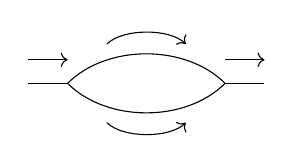
\begin{tikzpicture}
  \draw (0,1) --(-0.5,1);
  \draw[<-] (0,1.3) --(-0.5,1.3);
 \draw  (0,1) .. controls (0.5,1.5) and (1.5,1.5) .. (2,1);
  \draw [->](.5,1.5) .. controls (0.7,1.7) and (1.3,1.7) .. (1.5,1.5);
 \draw (0,1) .. controls (0.5,0.5) and (1.5,0.5) .. (2,1);
   \draw [->](.5,0.5) .. controls (0.7,0.3) and (1.3,0.3) .. (1.5,.5);
 \draw (2,1) --(2.5,1);
 \draw[->] (2,1.3) --(2.5,1.3);
 \end{tikzpicture}\;\;\;\;\;\;\;\;
 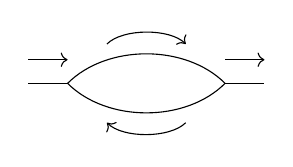
\begin{tikzpicture}
  \draw (0,1) --(-0.5,1);
  \draw[<-] (0,1.3) --(-0.5,1.3);
 \draw  (0,1) .. controls (0.5,1.5) and (1.5,1.5) .. (2,1);
  \draw [->](.5,1.5) .. controls (0.7,1.7) and (1.3,1.7) .. (1.5,1.5);
 \draw (0,1) .. controls (0.5,0.5) and (1.5,0.5) .. (2,1);
   \draw [<-](.5,0.5) .. controls (0.7,0.3) and (1.3,0.3) .. (1.5,.5);
 \draw (2,1) --(2.5,1);
 \draw[->] (2,1.3) --(2.5,1.3);
 \end{tikzpicture}\;\;\;\;\;\;\;\;
 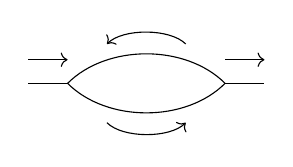
\begin{tikzpicture}
  \draw (0,1) --(-0.5,1);
  \draw[<-] (0,1.3) --(-0.5,1.3);
 \draw  (0,1) .. controls (0.5,1.5) and (1.5,1.5) .. (2,1);
  \draw [<-](.5,1.5) .. controls (0.7,1.7) and (1.3,1.7) .. (1.5,1.5);
 \draw (0,1) .. controls (0.5,0.5) and (1.5,0.5) .. (2,1);
   \draw [->](.5,0.5) .. controls (0.7,0.3) and (1.3,0.3) .. (1.5,.5);
 \draw (2,1) --(2.5,1);
 \draw[->] (2,1.3) --(2.5,1.3);
 \end{tikzpicture}\;,
 \caption{Possible energy flows of the self energy graph, (taking into account also all the inverted ones).}\label{muchachota}
 \end{figure}
 
 
 Of course the second and third flows from the left will give the same answer. In the first case, choosing $E_2$ and $E_3$ as independent energies, it is not necessary to invert the matrix $\mathfrak{B}$ since the region of integration is already $\mathbb{R}_+^2$. This energy flow gives the TOPT propagator
 \begin{equation}
 \frac{-1}{(-\Delta\tau+|\vec{z}_1|+|\Delta\vec{y}|+|\vec{z}_4|+i\eta)^2}\;,
 \end{equation}
 where $\Delta\tau\equiv x_2^0-x_1^0$ is the difference in time between the initial and final points and $\Delta \vec{y}\equiv\vec{z}_2=\vec{z}_3$. For the second energy flow above we have only one independent restriction, namely $E_2-E_3\geq0$. We construct the positive definite variables $y_i$ as
 \[
y=\mathfrak{B}E
=  \left(\begin{array}{@{}cc@{}}
-1 & 1\\
0 & 1
  \end{array}\right) \left(\begin{array}{@{}c@{}}
E_3\\
E_2
  \end{array}\right)\Rightarrow E=\left(\begin{array}{@{}cc@{}}
-1 & 1\\
0 & 1
  \end{array}\right) \left(\begin{array}{@{}c@{}}
y_1\\
y_2
  \end{array}\right)\;.
  \]
 Notice that we could not have chosen a positive definite variable $y_i=E_3$ since $d_3$ does not have the same sign as $d_3+\sum_kc_{k3} d'_k$ and the $i\eta$ part in the $E_3$ integration would not have the correct sign to carry out the Schwinger parametrization.\par
 We are ready to use (\ref{jetoraso}) to obtain the TOPT propagators as
 
 \begin{align}
 \prod_{l'=1}^{N_p}&\frac{-i}{\sum_l b_{ll'}d_l[\alpha^{-d_l}_l+\sum_k c_{kl}\alpha_k^{-d'_k}]}=\frac{-i}{(\alpha^{+}_3+\alpha^{-}_1+\alpha^{-}_4)}\nonumber\times\\
&\;\;\;\;\; \times\frac{-i}{(\alpha^{-}_2+\alpha^{-}_1+\alpha^{-}_4)-(\alpha^{+}_3+\alpha^{-}_1+\alpha^{-}_4)}\;,
\end{align}
giving
\begin{align}
 \frac{-1}{2(-\Delta\tau+|\vec{z}_1|-|\Delta \vec{y}|+|\vec{z}_4|+i\eta)(|\Delta\vec{y}|+i\eta)}\;.
 \end{align}


 Hence, adding all the contributions from the different energy flows
 

 
 
 
\begin{align}
&\Sigma_S(x_1,x_2)=\frac{g^2}{(2\pi)^6}\int d^3y_1d^3y_2\Big(\prod_{j=1}^4\frac{1}{2|\vec{z}_j|+i\eta}\Big)\times\nonumber\\
&\times\Big[\frac{1}{(-\Delta\tau+|\vec{z}_1|+|\Delta\vec{y}|+|\vec{z}_4|+i\eta)^2}+\frac{1}{(|\Delta\vec{y}|+i\eta)}\times\nonumber\\
 &\times\frac{1}{(-\Delta\tau+|\vec{z}_1|-|\Delta \vec{y}|+|\vec{z}_4|+i\eta)}+(\Delta\tau\leftrightarrow-\Delta\tau)\Big]\;,\label{roneo}
 \end{align}
 To interpret this result let us assume now that $x_1$ and $x_2$ are lightlike separated, i.e. $\Delta\tau=|\vec{x_2}|=|\vec{z}_1+\Delta \vec{y}+\vec{z}_4|$ (where we set $x_1=0$, and assume that $x_2$ has the largest time). To get a divergence from the first term between square brackets in (\ref{roneo}), the condition $\Delta\tau=|\vec{z}_1|+|\Delta \vec{y}|+|\vec{z}_4|$ must hold. These two conditions will be satisfied at the same time if and only if $\vec{z}_1\parallel\Delta \vec{y}\parallel \vec{z}_4$ and, to have that $|\vec{x}_2-\vec{x}_1|=|\vec{z}_1|+|\Delta \vec{y}|+|\vec{z}_4|$, if the two internal vertices are between the external ones with the one at $\vec{y}_1$ closer to $\vec{x}_1$ than the one at $\vec{y}_2$. In this that all lines flow spatially forward, corresponding to the momentum-space TOPT configuration in Fig. \ref{asddasdas} (a). Hence, this divergence is caused by the collinear configuration that we expect from the Coleman-Norton picture for this diagram, with the vertices ordered in space so that no lines emerge from the vacuum. Note however that we can only see the spatial configuration of the internal vertices but not say anything about the on-shell or off-shell condition of the internal lines (See Fig. \ref{kiolo}). This is just the trade we make, in momentum-space 
TOPT lines are on-shell but energy is not conserved at each vertex, in coordinate-space TOPT energy is conserved but there is no on-shell condition on the lines.\par
 In the timelike case, $\Delta\tau>|\vec{x}_2|$, the only restriction for a singularity is that the lines must not be collinear, however these divergences do not correspond to physical configurations in agreement with conservation of momentum. The spacelike case has $\Delta\tau<|\vec{x}_2|$ which can never be satisfied at the same time as $\Delta\tau=|\vec{z}_1|+|\Delta \vec{y}|+|\vec{z}_4|$, not giving rise to divergences coming from denominators.
 
  \begin{figure}[ht!]
 \centering
%  \begin{tikzpicture}
%  \draw (0,0) --(1.5,1.5);
%    \draw (0,0) --(-1.5,1.5);
%    \draw(0,1.5) ellipse (42.6pt and 4pt);
 %   \path[draw=blue, dashed] (0,0) -- (0.4,0.2) -- (1,1.1) -- (1.3,1.3);
%    \draw (0.4,0.19) node {$\cdot$};
 %       \draw (1,1.09) node {$\cdot$};
%       \draw (1.3,1.29) node {$\cdot$};
 %      \draw (0.4,0.39) node {$\cdot$};
%       \draw (1.,.99) node {$\cdot$};
%\draw (1.6,0.75) node {\tiny$\Delta\tau$};
%       \draw (0,-0.12) node {\tiny$\vec{x}_1$};
 %      \draw[|<->|] (1.3,-0.007) -- (1.3,1.3);
%       \draw[dotted] (0,0)--(1.3,0);
%       \draw[green,dashed] (0,0)--(1.3,1.3);
%\draw (1.3,-0.12) node {\tiny$\vec{x}_2$};
%\path[draw=red, dashed] (0,0) -- (0.2,0.3) -- (-0.3,0.6) -- (1.3,1.3);
 %\draw (0.2,0.29) node {$\cdot$};
%  \draw (-0.3,0.59) node {$\cdot$};
%      \draw[ultra thin](0,0.27) ellipse (7.3pt and 1.5pt);
 %      \draw[ultra thin] (0,0.84) ellipse (24pt and 2.2pt);
 %\end{tikzpicture}\;\;\;\;\;\;\;\;\;\;\;\;
   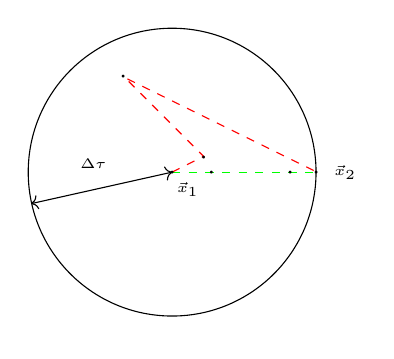
\begin{tikzpicture}[ scale=2]
   \draw (0,0) ellipse (26pt and 26pt);
   \path[draw=red, dashed] (0,0) -- (0.2,0.1) -- (-0.3,0.6) -- (0.92,0);
    \draw[green,dashed] (0,0)--(0.9,0);
 \draw (0.2,0.09) node {$\cdot$};   
  \draw (-0.31,0.6) node {$\cdot$};    
    \draw (0.915,-0.01) node {$\cdot$};    
        \draw (0,-0.01) node {$\cdot$};   
                \draw (0.25,-0.01) node {$\cdot$};    
                 \draw (0.75,-0.01) node {$\cdot$};    
   \draw (-0.5,0.05) node {\tiny$\Delta\tau$};
   \draw[<->] (-0.895,-0.2) -- (0,0);
   \draw (1.1,0) node {\tiny$\vec{x}_2$};
    \draw (0.1,-0.11) node {\tiny$\vec{x}_1$};
    \draw (0,-0.95) node {$\;$};
   \end{tikzpicture}
 \caption{ Space representation of some of the configurations for the scalar self energy diagram with lightlike separated endpoints $\vec{x}_1$ and $\vec{x}_2$. The red path does not give a divergence for the first term inside square brackets in (\ref{roneo}), while the green path does. Seeing therefore that collinear configurations are allowed to give divercencies.}\label{kiolo}
 \end{figure}
 
 Let us study the second term in (\ref{roneo}), which we will call $\Sigma^{hsc}_S$, using the Feynman parametrization. This amounts to
 \begin{align}
 &\Sigma^{hsc}_S=\frac{g^2}{(2\pi)^6}\int d^3y_1d^3y_2\Big(\prod_{j=1}^4\frac{1}{2|\vec{z}_j|+i\eta}\Big)\times\nonumber\\
&\times \int_0^1 \frac{d\alpha}{[(1-\alpha)(-\Delta\tau+|\vec{z}_1|-|\Delta\vec{y}|+|\vec{z}_4|)+\alpha|\Delta\vec{y}|+i\eta]^2} \;.\label{yeeva}
 \end{align}
 Notice that the type of denominators appearing in coordinate-space TOPT are linear in the coordinates of the vertices so that we will only have endpoint singularities, i.e. when $\alpha_j=0$, when the argument of each denominator vanishes, or when the vertices are placed at infinity. Looking at (\ref{yeeva}), one could argue that the denominators $1/2|z_j|$ should also appear in the Feynman parametrization. And this is true, but since we have only endpoint singularities these will represent two vertices going hard, $|\vec{z}_j|=0$ if the corresponding Feynman parameter is one (forcing also all the other parameters to be set to zero due to the delta function $\delta(1-\Sigma_i\alpha_i)$ from the parametrization), and will not contribute to the denominator when the corresponding $\alpha_j$ is zero. The parametrized term in (\ref{yeeva}) tells us that, when $\alpha=1$, we will have a hard singularity if $|\Delta y|=0$, while the path between the external points is not restricted to be lightlike and to have collinear internal vertices. If $\alpha=0$ we are dealing with a possible soft divergence (remember the identification $\lambda\alpha\Delta \vec{y}=\vec{p}$, so that the line will carry zero momentum but with a finite displacement). In this case, taking the external points as lightlike separated (i.e. $\Delta\tau=|\vec{x_2}|$), a collinear pinch surface appears in the configurations in Fig. \ref{Heto}.
 \begin{figure}[ht!]
 \centering
 \begin{tikzpicture}
 To do
\end{tikzpicture}

\centering
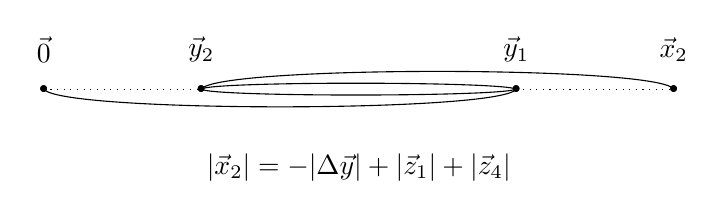
\begin{tikzpicture}
\draw (2,0) node {\tiny$\bullet$};
\draw (6,0) node {\tiny$\bullet$};
\draw (2,0) .. controls (2.1,-0.1) and (5.8,-.1) .. (6,0);
\draw (2,0) .. controls (2.1,0.1) and (5.8,.1) .. (6,0);
\draw (0,0)node {\tiny$\bullet$};
\draw (8,0) node {\tiny$\bullet$};
\draw[dotted,thin] (0,0)node {\tiny$\bullet$} -- (2,0) node {\tiny$\bullet$};
\draw[dotted,thin] (6,0)node {\tiny$\bullet$} -- (8,0) node {\tiny$\bullet$};
\draw (0,0.5)node {$\vec{0}$};
\draw (8,0.5)node {$\vec{x}_2$};
\draw (2,0.5)node {$\vec{y}_2$};
\draw (6,0.5)node {$\vec{y}_1$};
\draw (4,-1)node {$|\vec{x}_{2}|=-|\Delta\vec{y}|+|\vec{z}_1|+|\vec{z}_4|$};
\draw (0,0) .. controls (.2,-0.3) and (5.8,-.3) .. (6,0);
\draw (2,0) .. controls (2.2,0.3) and (7.8,.3) .. (8,0);
\end{tikzpicture}
\caption{Soft-collinear configurations giving rise to possible divergences of the coordinate-space TOPT self energy diagram in equation (\ref{roneo}). One can see that these configuration corresponds to the one in Fig. \ref{asddasdas} (b) studied in the momentum-space TOPT, where lines emerged from the vacuum.}\label{Heto}
\end{figure}
 
At this point, we have to power-count the different divergences to analyze if they correspond to true singularities. Recall that from the momentum-space  covariant version of the scalar self-energy diagram we expect logarithmic UV hard and collinear divergences but no soft divergences. Let us analyze the first type of divergence that arises when $\Delta \vec{y}\to 0$. Assuming that now $\Delta\tau\neq|\vec{z}_1|+|\vec{z}_4|$ to avoid the zeroth-order lightcone divergences (coming from the first denominator in the second term of (\ref{roneo})), we have that the term from (\ref{roneo}) encoding the UV hard divergence is proportional to
 \begin{align}
 I\equiv&\int dy_1^1dy_1^2dy_1^3dy_2^1dy_2^2dy_2^3\Big(\frac{1}{|\sum_{i=1}^3(y_2^i-y_1^i)^2|^{\frac{1}{2}}}\Big)^3\times\nonumber\\
 &\times\frac{f(\{y_i^j\})}{(-\Delta\tau+|\vec{z}_1|+|\vec{z}_4|+i\eta)}\nonumber=\\
 =&\int dy_+^1dy_+^2dy_+^3dy_-^1dy_-^2dy_-^3\Big(\frac{1}{2|\sum_{i=1}^3(y_-^i)^2|^{\frac{1}{2}}}\Big)^3\times\nonumber\\
 &\times\frac{f(\{y_i^j\})}{(-\Delta\tau+|\vec{z}_1|+|\vec{z}_4|+i\eta)}
 \end{align}
 where we define $y_\pm^i=y_2^i\pm y_1^i$ (the $y^i$ are the spatial coordinates of each vertex) and $f(\{y_i^j\})$ is a finite function at the pinch surface containing all remaining terms for this contribution in (\ref{assuca}). We rescale $y_-^i\to\lambda y_-^i$ so that we reach the hard limit when $\lambda=0$. It is easy now to see that with this rescaling the integral scales as $\lambda^0$ so that the overall degree of divergence of the diagram is logarithmic as we had for the covariant diagram. We will not power count the other divergencies in this case, since we do in the next example.
 
  %Remember also that we have to recover these degrees of divergence after extracting the divergence coming from setting the external points on each other's lightcone. 
 
 
 %Next, let us use the LTE to identify the imaginary parts of the diagram. Taking $x_2^0$ to be the largest time, the following diagrammatic identities hold
 %\begin{equation}
 %\begin{tikzpicture}
 % \draw (0,1) --(-0.5,1);
 %\draw (0,1) .. controls (0.5,1.5) and (1.5,1.5) .. (2,1);
 %\draw (0,1) .. controls (0.5,0.5) and (1.5,0.5) .. (2,1);
 %\draw (2,1) --(2.5,1);
 % \draw (3,.97) node {$=$};
 % \draw (0,0.13) node {$\;$};
 %\end{tikzpicture}
 % \begin{tikzpicture}
 % \draw (0,1) --(-0.5,1);
 %\draw (0,1) .. controls (0.5,1.5) and (1.5,1.5) .. (2,1);
 %\draw (0,1) .. controls (0.5,0.5) and (1.5,0.5) .. (2,1);
 %\draw (2,1) --(2.5,1);
% \draw (2.5,0.99) node {$\tiny\cdot$};
%    \draw (2.5,1) ellipse (3pt and 3pt);
%  \draw (0,0.13) node {$\;$};
%    \draw (-1,.99) node {$-$};
% \end{tikzpicture}
%  \begin{tikzpicture}
%  \draw (0,1) --(-0.5,1);     
%   \draw (-1,.99) node {$\;\;;$};
 %    \draw (-0.5,0.99) node {$\tiny\cdot$};
 %   \draw (-0.5,1) ellipse (3pt and 3pt);

% \draw (0,1) .. controls (0.5,1.5) and (1.5,1.5) .. (2,1);
 %\draw (0,1) .. controls (0.5,0.5) and (1.5,0.5) .. (2,1);
 %\draw (2,1) --(2.5,1);
 % \draw (2,0.99) node {$\tiny\cdot$};
 %   \draw (2,1) ellipse (3pt and 3pt);
 %    \draw (0,0.99) node {$\tiny\cdot$};
%    \draw (0,1) ellipse (3pt and 3pt);
%      \draw (2.5,0.99) node {$\tiny\cdot$};
 %   \draw (2.5,1) ellipse (3pt and 3pt);
 % \draw (3,.97) node {$=$};
 % \draw (0,0.13) node {$\;$};
 %\end{tikzpicture}
%  \begin{tikzpicture}
%  \draw (0,1) --(-0.5,1);
% \draw (0,1) .. controls (0.5,1.5) and (1.5,1.5) .. (2,1);
% \draw (0,1) .. controls (0.5,0.5) and (1.5,0.5) .. (2,1);
% \draw (2,1) --(2.5,1);
%   \draw (2,0.99) node {$\tiny\cdot$};
%    \draw (2,1) ellipse (3pt and 3pt);
 %     \draw (0,0.99) node {$\tiny\cdot$};
 %   \draw (0,1) ellipse (3pt and 3pt);
%      \draw (-0.5,0.99) node {$\tiny\cdot$};
%    \draw (-0.5,1) ellipse (3pt and 3pt);

%  \draw (0,0.13) node {$\;$};
%    \draw (-1,.99) node {$-$};
 %      \draw (2.6,.99) node {$\;.$};
% \end{tikzpicture}
% \end{equation}
%Summing the first diagram and its complex conjugate, which is the third diagram above, we will obtain two times the imaginary part of the diagram (remember all the diagrams have an extra $i$ to contribute to the $T$ matrix). So that
%\begin{align}
%\centering
%&\begin{tikzpicture}
%\draw (-1,0) node {$2\text{Im}$};
%  \draw (0,0) --(-0.5,0);
% \draw (0,0) .. controls (0.5,0.5) and (1.5,0.5) .. (2,0);
% \draw (0,0) .. controls (0.5,-0.5) and (1.5,-0.5) .. (2,0);
 %\draw (2,0) --(2.5,0);
 %\end{tikzpicture}
 %   \begin{tikzpicture}
%      \draw (0,0) --(-0.5,0);
% \draw (0,0) .. controls (0.5,0.5) and (1.5,0.5) .. (2,0);
 %\draw (0,0) .. controls (0.5,-0.5) and (1.5,-0.5) .. (2,0);
 %\draw (2,0) --(2.5,0);
 %\draw (2.5,-0.01) node {$\tiny\cdot$};
 %   \draw (2.5,0) ellipse (3pt and 3pt);
 % \draw (0,0.13) node {$\;$};
 %   \draw (-1,-0.01) node {$=\;-\;$};
%    \end{tikzpicture}
%     \begin{tikzpicture}
%   \draw (0,1) --(-0.5,1);
% \draw (0,1) .. controls (0.5,1.5) and (1.5,1.5) .. (2,1);
% \draw (0,1) .. controls (0.5,0.5) and (1.5,0.5) .. (2,1);
% \draw (2,1) --(2.5,1);
%   \draw (2,0.99) node {$\tiny\cdot$};
 %   \draw (2,1) ellipse (3pt and 3pt);
 %     \draw (0,0.99) node {$\tiny\cdot$};
 %   \draw (0,1) ellipse (3pt and 3pt);
%      \draw (-0.5,0.99) node {$\tiny\cdot$};
%    \draw (-0.5,1) ellipse (3pt and 3pt);
 %    \draw (-1,.99) node {$-$};  \draw (3,1) node {$\propto$};
 %   \end{tikzpicture}\nonumber\\
 %   &\propto\int d^4y_1 d^4y_2\Big(\Delta(y_1-x_1)\Delta^2(y_2-y_1)\Delta^+(x_2-y_2)+\Delta^\ast(y_1-x_1){\Delta^\ast}^2(y_2-y_1)\Delta^-(x_2-y_2)\Big)\;.
% \end{align}
 %Now let us study the two possible time orderings of the internal vertices assuming $x_1^0<y_1^0,y_2^0<x_2^0$. In the case $y_2^0>y_1^0$ we can substitute the Feynman propagators by the $\Delta^+$ and their complex conjugates by $\Delta^-$, obtaining
 %\begin{align}
%&\begin{tikzpicture}
%\draw (-1,0) node {$2\text{Im}$};
%  \draw (0,0) --(-0.5,0);
% \draw (0,0) .. controls (0.5,0.5) and (1.5,0.5) .. (2,0);
% \draw (0,0) .. controls (0.5,-0.5) and (1.5,-0.5) .. (2,0);
% \draw (2,0) --(2.5,0);
% \draw (3.5,-0.1) node {$\propto_{y_2^0>y_1^0}$};
% \end{tikzpicture}\nonumber\\
%    &\propto\int d^4y_1 d^4y_2\Big(\Delta^+(y_1-x_1){\Delta^+}^2(y_2-y_1)\Delta^+(x_2-y_2)+\Delta^-(y_1-x_1){\Delta^-}^2(y_2-y_1)\Delta^-(x_2-y_2)\Big)\;.\label{yeva}
 %\end{align}
 
%For the other time ordering $y_2^0<y_1^0$ we will have
% \begin{align}
%&\begin{tikzpicture}
%\draw (-1,0) node {$2\text{Im}$};
 % \draw (0,0) --(-0.5,0);
 %\draw (0,0) .. controls (0.5,0.5) and (1.5,0.5) .. (2,0);
 %\draw (0,0) .. controls (0.5,-0.5) and (1.5,-0.5) .. (2,0);
 %\draw (2,0) --(2.5,0);
% \draw (3.5,-0.1) node {$\propto_{y_2^0<y_1^0}$};
% \end{tikzpicture}\nonumber\\
%    &\propto\int d^4y_1 d^4y_2\Big(\Delta^+(y_1-x_1){\Delta^-}^2(y_2-y_1)\Delta^+(x_2-y_2)+\Delta^-(y_1-x_1){\Delta^+}^2(y_2-y_1)\Delta^-(x_2-y_2)\Big)\;.\label{yeva2}
% \end{align}
%Remembering that the $\Delta^\pm$ are propagators of on-shell particles with positive or negative frequency, we see that the imaginary part of this diagram arises when particles travel on-shell between vertices. Also, the $\Delta^\pm$ tell us how the energy flows with respect to the time ordering. In the first term of (\ref{yeva}) we see how all the energy flows forward in time, corresponding to the configuration in Fig. \ref{asddasdas} (a), and that the second term has the opposite energy flow. In the other case, the first term in (\ref{yeva2}) tells us that the energy flows forward in time from $x_1$ to $y_1$ and from $y_2$ to $x_2$, and backwards from $y_1$ to $y_2$, corresponding to the configuration in Fig. \ref{asddasdas} (b) and the coordinate-space counterpart in Fig. \ref{Heto} where three particles emerged from the vacuum and two of them annihilate with the incoming particle and the other travels to the final state.\par

\subsubsection{Scalar one-loop vertex diagram}

Let us move on to a more relevant example that has connections with all the previous discussions, i.e. the triangle diagram in Fig. \ref{lanroni}.

\begin{figure}[ht!]
\centering
\begin{tikzpicture}
\begin{feynman}
\vertex (a);
\vertex [left=1.3 cm of a] (b);
\vertex [left=.02 cm of b] (b113311){$x_1$};
\vertex [left=1.1 cm of a] (b1111){\tiny$\bullet$};
\vertex [right=1.12 cm of b] (b1111){\tiny$\bullet$};
\vertex [right=0.3 cm of b1111] (111c1){$y_1$};
\vertex [above right=1.3 cm of a] (c);
\vertex [above right=1.3 cm of c] (chh);
\vertex [ right=0.1 cm of chh] (chh444){$x_3$};
\vertex [above right=1.05 cm of c] (chhs){\tiny$\bullet$};
\vertex [above=0.01 cm of c] (chhs222){$y_3$};
\vertex [below right=1.3 cm of a] (c2);
\vertex [below right=1.3 cm of c2] (c2hh);
\vertex [below =.01 cm of c2] (c2kkkkk){$y_2$};
\vertex [right=.1 cm of c2hh] (c2hhww){$x_2$};
\vertex [below right=1.05 cm of c2] (c2hhss){\tiny$\bullet$};
\vertex [below right=1.05 cm of a] (c222){\tiny$\bullet$};
\vertex [above right=1.05 cm of a] (c222){\tiny$\bullet$};
\vertex [right=2.5 cm of a] (heheheheheh) {$\equiv ig\Gamma_S(x_1,x_2,x_3)$};






\diagram* {
(b)-- [fermion, edge label=1](a)
(a)-- [fermion, edge label=3](c)
(c2hh)-- [edge label=5](c2)
(c)-- [fermion,edge label=6](chh)
(c2)-- [fermion](c2hh)
(a)-- [fermion](c2)
(c2)-- [edge label=2](a)
(c2)-- [fermion](c)
(c)-- [edge label=4](c2)
};
\end{feynman}
\end{tikzpicture}
\caption{Coordinate representation of the scalar triangle diagram. With this choice of where the lines start and end, the non zero elements of the incidence matrices are: $\epsilon_{11}=\epsilon_{22}=\epsilon_{33}=\epsilon_{43}=\epsilon'_{63}=\epsilon'_{52}=+1$ and $\epsilon'_{11}=\epsilon_{21}=\epsilon_{31}=\epsilon_{52}=\epsilon_{42}=\epsilon_{63}=-1$. }\label{lanroni}
\end{figure}

Reading from Fig. \ref{yuero} and using (\ref{dadada444}) we have that
\begin{align}
 \Gamma_S(x_1,x_2,x_3)&=\frac{-ig^2}{(2\pi)^9}\int\prod_{i=1}^3d^3y_i\prod_{j=1}^6\int_{-\infty}^{+\infty}{dE^0_j}\times\nonumber\\
&\times\frac{f_j(E_j)}{2|{\vec{z}_j}|+i\eta}\prod_{i=1}^3\delta\Big(\sum_{l=1}^6E_{l}^0\epsilon_{li}\Big)\nonumber\equiv\\
 &\equiv\frac{-g^2}{(2\pi)^9}\int\prod_{i=1}^3d^3y_i\varUpsilon_S(\{y_i\})\;.\label{heil}
\end{align}
After a very lengthy calculation, from the possible 64 terms ( corresponding to the possible energy flows) we are left with only 24 non-trivial energy flows. Using the Schwinger parametrization, these yield the result (omitting the $i\eta$s)
\begin{align}
 &\Gamma_S(x_1,x_2,x_3)=-\frac{g^2}{(2\pi)^9}\int\prod_{i=1}^3d^3y_i\Big(\prod_{j=1}^6\frac{1}{2|\vec{z_j}|+i\eta}\Big)\Big\{\Big[\sum_{\{I,p_1,p_2\}} \nonumber\\
 &\frac{1}{-\Delta\tau_{31}+|\vec{z}_1|+|\vec{z}_3|+|\vec{z}_6|}\frac{1}{-\Delta\tau_{31}+|\vec{z}_1|+|\vec{z}_2|+|\vec{z}_4|+|\vec{z}_6|}\nonumber\times\\
& \times \Big(\frac{1}{-\Delta\tau_{2,13}+|\vec{z}_5|+\frac{1}{2}(|\vec{z}_1|+|\vec{z}_2|-|\vec{z}_4|-|\vec{z}_6|)}+\nonumber\\
&+\frac{1}{\Delta\tau_{2,13}+|\vec{z}_5|+\frac{1}{2}(-|\vec{z}_1|-|\vec{z}_2|+|\vec{z}_4|+|\vec{z}_6|)}\Big)\Big]+\nonumber\\
%&+\frac{1}{-\Delta\tau_{21}+|\vec{z}_1|+|\vec{z}_2|+|\vec{z}_5|+i\eta}\frac{1}{-\Delta\tau_{21}+|\vec{z}_1|+|\vec{z}_3|+|\vec{z}_4|+|\vec{z}_5|+i\eta}\times\nonumber\\
%&\times\Big(\frac{1}{-\Delta\tau_{3,12}+|\vec{z}_6|+\frac{1}{2}(|\vec{z}_1|+|\vec{z}_3|-|\vec{z}_4|-|\vec{z}_5|)+i\eta}+\frac{1}{\Delta\tau_{3,12}+|\vec{z}_6|+\frac{1}{2}(-|\vec{z}_1|-|\vec{z}_3|+|\vec{z}_4|+|\vec{z}_5|)+i\eta}\Big)\nonumber\\
%&+\frac{1}{-\Delta\tau_{32}+|\vec{z}_4|+|\vec{z}_5|+|\vec{z}_6|+i\eta}\frac{1}{-\Delta\tau_{32}+|\vec{z}_2|+|\vec{z}_3|+|\vec{z}_5|+|\vec{z}_6|+i\eta}\times\nonumber\\
%&\times\Big(\frac{1}{-\Delta\tau_{1,32}+|\vec{z}_1|+\frac{1}{2}(|\vec{z}_2|-|\vec{z}_3|+|\vec{z}_5|-|\vec{z}_6|)+i\eta}+\frac{1}{\Delta\tau_{1,32}+|\vec{z}_1|+\frac{1}{2}(-|\vec{z}_2|+|\vec{z}_3|-|\vec{z}_5|+|\vec{z}_6|)+i\eta}\Big)\nonumber\\
&+\frac{1}{|\vec{z}_2|+|\vec{z}_3|+|\vec{z}_4|}\Big[\frac{1}{-\Delta\tau_{31}+|\vec{z}_1|+|\vec{z}_6|+\frac{1}{2}(-|\vec{z}_2|+|\vec{z}_3|-|\vec{z}_4|)}\times\nonumber\\
&\times\Big(\frac{1}{-\Delta\tau_{32}-|\vec{z}_4|+|\vec{z}_5|+|\vec{z}_6|}+\frac{1}{-\Delta\tau_{21}+|\vec{z}_1|-|\vec{z}_2|+|\vec{z}_5|}\Big)+\nonumber\\
&+\frac{1}{-\Delta\tau_{32}+|\vec{z}_5|+|\vec{z}_6|+\frac{1}{2}(-|\vec{z}_2|-|\vec{z}_3|+|\vec{z}_4|)}\times\nonumber\\
&\Big(\frac{1}{-\Delta\tau_{12}+|\vec{z}_1|-|\vec{z}_2|+|\vec{z}_5|}+\frac{1}{-\Delta\tau_{31}+|\vec{z}_1|-|\vec{z}_3|+|\vec{z}_6|}\Big)+\nonumber\\
&\frac{1}{-\Delta\tau_{12}+|\vec{z}_1|+|\vec{z}_5|+\frac{1}{2}(|\vec{z}_2|-|\vec{z}_3|-|\vec{z}_4|)}\times\nonumber\\
&\times\Big(\frac{1}{-\Delta\tau_{32}-|\vec{z}_4|+|\vec{z}_5|+|\vec{z}_6|}+\frac{1}{-\Delta\tau_{13}+|\vec{z}_1|-|\vec{z}_3|+|\vec{z}_6|}\Big)\Big]+\nonumber\\
&+(\tau\leftrightarrow-\tau)\Big\}\;.\label{assuca}
 \end{align}
 Where we define, $\Delta\tau_{i,jk}=x_i^0-\frac{1}{2}(x_j^0+x_k^0)$, and the last symbol in brackets represents the terms shown before it with an extra minus sign in all the time components. The sum in the first square brackets runs in the permutations of labels in the following way: the identity $I$ does nothin, $p_1$ interchanges $(|\vec{z}_2|,|\vec{z}_5|,x_2^0)\leftrightarrow(|\vec{z}_3|, |\vec{z}_6|,x_3^0)$, and $p_2$ interchanges $(|\vec{z}_2|,|\vec{z}_5|,x_1^0)\leftrightarrow(|\vec{z}_3|, |\vec{z}_6|,x_2^0)$.\par
 Let us interpret the divergences coming from the different terms above assuming all external points are lightlike separated between them. The first term between curly brackets above can be expressed as,  
 \begin{align}
&\frac{1}{-\Delta\tau_{31}+|\vec{z}_1|+|\vec{z}_3|+|\vec{z}_6|}\frac{1}{-\Delta\tau_{31}+|\vec{z}_1|+|\vec{z}_2|+|\vec{z}_4|+|\vec{z}_6|}\nonumber\\
&\times\frac{2}{-\Delta\tau_{21}+|\vec{z}_5|+|\vec{z}_1|+|\vec{z}_2|-\Delta\tau_{23}+|\vec{z}_5|-|\vec{z}_4|-|\vec{z}_6|}\label{jejejeje}\;.
\end{align}
 We see that the first two TOPT propagators, in case $\Delta\tau_{31}>0$, will give rise to divergences whenever the three internal vertices lie in the direction between $\vec{x}_1$ and $\vec{x}_3$ ordered as $\vec{y}_1$-$\vec{y}_2$-$\vec{y}_3$, in this direction. The third propagator will give another divergence when $\vec{x}_2$ lies in the direction of $\vec{x}_3-\vec{x}_1$ and after $\vec{x}_3$ if $\Delta\tau_{23}>0$, being all lines of the diagram collinear. See Fig. \ref{fueraya}.
 \begin{figure}[ht!]
\centering
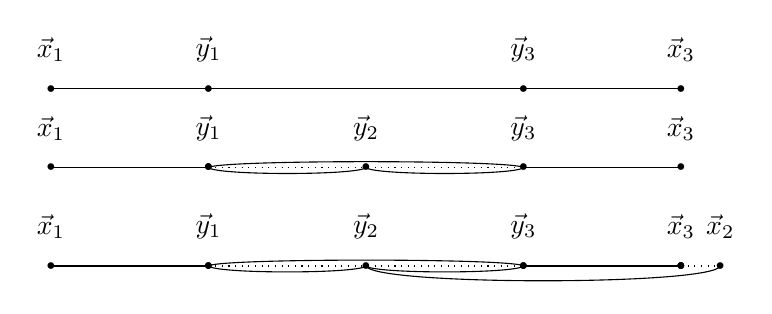
\begin{tikzpicture}
\draw (0,0)node {\tiny$\bullet$} -- (2,0) node {\tiny$\bullet$} -- (6,0) node {\tiny$\bullet$} -- (8,0) node {\tiny$\bullet$};
\draw (0,-1)node {\tiny$\bullet$} -- (2,-1) node {\tiny$\bullet$};
\draw[dotted] (2,-1) node {\tiny$\bullet$} -- (6,-1) node {\tiny$\bullet$};
\draw (4,-1) node {\tiny$\bullet$};
\draw (6,-1) -- (8,-1) node {\tiny$\bullet$};
\draw (0,-2.25)node {\tiny$\bullet$} -- (2,-2.25) node {\tiny$\bullet$};
\draw (6,-2.25) node {\tiny$\bullet$} -- (8,-2.25) node {\tiny$\bullet$};
\draw[dotted] (2,-2.25) node {\tiny$\bullet$} -- (6,-2.25) node {\tiny$\bullet$};
\draw (4,-2.25) node {\tiny$\bullet$};
\draw (6,-2.25) -- (8,-2.25) node {\tiny$\bullet$};
\draw (2,-1) .. controls (2.1,-0.9) and (5.9,-0.9) .. (6,-1);
\draw (2,-2.25) .. controls (2.1,-2.15) and (5.9,-2.15) .. (6,-2.25);
\draw (2,-1) .. controls (2.1,-1.1) and (3.9,-1.1) .. (4,-1);
\draw (4,-1) .. controls (4.1,-1.1) and (5.9,-1.1) .. (6,-1);
\draw (2,-2.25) .. controls (2.1,-2.35) and (3.9,-2.35) .. (4,-2.25);
\draw (4,-2.25) .. controls (4.1,-2.35) and (5.9,-2.35) .. (6,-2.25);
\draw (4,-2.25) .. controls (4.1,-2.5) and (8.4,-2.5) .. (8.5,-2.25);
\draw[thin,dotted] (8,-2.25) node {\tiny$\bullet$} --(8.5,-2.25) node {\tiny$\bullet$} ;
\draw (0,0.5)node {$\vec{x}_1$};
\draw (0,-0.5)node {$\vec{x}_1$};
\draw (8,-0.5)node {$\vec{x}_3$};
\draw (0,-1.75)node {$\vec{x}_1$};
\draw (8,-1.75)node {$\vec{x}_3$};
\draw (8,0.5)node {$\vec{x}_3$};
\draw (2,0.5)node {$\vec{y}_1$};
\draw (6,0.5)node {$\vec{y}_3$};
\draw (2,-0.5)node {$\vec{y}_1$};
\draw (6,-0.5)node {$\vec{y}_3$};
\draw (2,-1.75)node {$\vec{y}_1$};
\draw (6,-1.75)node {$\vec{y}_3$};
\draw (4,-1.75)node {$\vec{y}_2$};
\draw (4,-0.5)node {$\vec{y}_2$};
\draw (8.5,-1.75)node {$\vec{x}_2$};


\end{tikzpicture}
\caption{From top to bottom, the space collinear configurations giving rise to divergences in the first, second and third term in (\ref{jejejeje}) respectively. The external vertices are time-ordered from left to right. Notice that the first configuration (which gives $|(\vec{x}_{3}-\vec{x}_1)|=|\vec{z}_1|+|\vec{z}_3|+|\vec{z}_6|$) can happen independently of the other two, if we have the second configuration (giving $|(\vec{x}_{3}-\vec{x}_1)|=|\vec{z}_1|+|\vec{z}_2|+|\vec{z}_4|+|\vec{z}_6|$) we also have the first, and having the third (producing $|(\vec{x}_{2}-\vec{x}_1)|=|\vec{z}_1|+|\vec{z}_2|+|\vec{z}_5|$ and $|(\vec{x}_{2}-\vec{x}_3)|=|\vec{z}_5|-|\vec{z}_4|-|\vec{z}_6|$) means having also the previous two. The dotted line is depicted to represent the vertices being collinear.}\label{fueraya}
\end{figure}

 \begin{figure}[ht!]
\centering
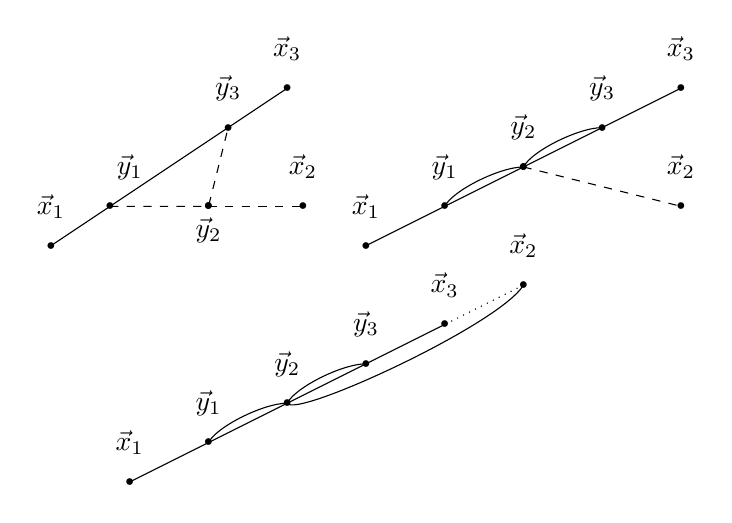
\begin{tikzpicture}
\draw (0,0)node {\tiny$\bullet$} -- (.75,.5) node {\tiny$\bullet$} -- (2.25,1.5) node {\tiny$\bullet$} -- (3,2) node {\tiny$\bullet$};
\draw[dashed] (0.75,.5) -- (2,0.5) node {\tiny$\bullet$} -- (2.25,1.5);
\draw[dashed] (2,0.5) node {\tiny$\bullet$} -- (3.2,0.5) node {\tiny$\bullet$};
\draw (4,0)node {\tiny$\bullet$} -- (5,.5) node {\tiny$\bullet$}--(6,1) node {\tiny$\bullet$} -- (7,1.5) node {\tiny$\bullet$} -- (8,2) node {\tiny$\bullet$};
\draw[dashed] (6,1) node {\tiny$\bullet$}--(8,0.5) node {\tiny$\bullet$};
\draw (1,-3)node {\tiny$\bullet$} -- (2,-2.5) node {\tiny$\bullet$}-- (3,-2) node {\tiny$\bullet$} -- (4,-1.5) node {\tiny$\bullet$} -- (5,-1) node {\tiny$\bullet$};
\draw[thin,dotted] (6,-0.5)--(5,-1);
\draw(6,-0.5) node {\tiny$\bullet$};
\draw (5,.5) .. controls (5.1,.7) and (5.7,1.) .. (6,1);
\draw (6,1) .. controls (6.1,1.2) and (6.7,1.5) .. (7,1.5);
\draw (2,-2.5) .. controls (2.1,-2.3) and (2.7,-2) .. (3,-2);
\draw (3,-2) .. controls (3.1,-1.8) and (3.7,-1.5) .. (4,-1.5);
\draw (3,-2) .. controls (3.1,-2.2) and (5.7,-1) .. (6,-.5);
\draw (1,-2.5) node {$\vec{x}_1$};
\draw (2,-2) node {$\vec{y}_1$};
\draw (3,-1.5) node {$\vec{y}_2$};
\draw (4,-1) node {$\vec{y}_3$};
\draw (5,-0.5) node {$\vec{x}_3$};
\draw (8,1) node {$\vec{x}_2$};
\draw (6,0) node {$\vec{x}_2$};
\draw (0,0.5)node {$\vec{x}_1$};
\draw (1,1)node {$\vec{y}_1$};
\draw (2.25,2)node {$\vec{y}_3$};
\draw (3,2.5)node {$\vec{x}_3$};
\draw (4,0.5)node {$\vec{x}_1$};
\draw (5,1)node {$\vec{y}_1$};
\draw (6,1.5)node {$\vec{y}_2$};
\draw (7,2)node {$\vec{y}_3$};
\draw (8,2.5)node {$\vec{x}_3$};
\draw (3.2,1)node {$\vec{x}_2$};
\draw (2,0.2)node {$\vec{y}_2$};
\end{tikzpicture}
\caption{The three configurations for the vertex diagram giving rise to divergences in (\ref{jejejeje}).  The dashed lines are free while the bold lines are fixed in that particular configuration. Meaning that in the first diagram from the left $\vec{y}_2$ and $\vec{x}_2$ can be placed anywhere in space, still giving rise to a divergence in the first term in (\ref{jejejeje}) no matter the time ordering of $\vec{x}_2$. In the second diagram only $\vec{x}_2$ is free (and also its time ordering with respect to the other vertices), giving divergences in the first and second term in (\ref{jejejeje}). In the third diagram all vertices must be collinear and the external vertices are time ordered from left to right, giving rise to a divergence in all the terms in (\ref{jejejeje}).}\label{fueraya2}
\end{figure}
Let us power-count these collinear divergences to see if they correspond to true singularities. Remember that from the Coleman-Norton picture for this diagram we expect divergences coming from configurations with the topologies in Fig. \ref{fig:reddiag} (b)-(c) and we will see appear also (d) since in our scalar theory it is the same as the other ones. We will require that $\vec{x}_2$ is not collinear to $\vec{x}_3-\vec{x}_1$, so that the divergence from the third configuration in the figure above is not present, and by translational invariance we can set $\vec{x}_{1}=\vec{0}$. To power-count we will use cylindrical coordinates with $\vec{x}_3$ oriented in the $z$-axis in Fig. \ref{frens}. 
\begin{figure}[ht!]
\centering
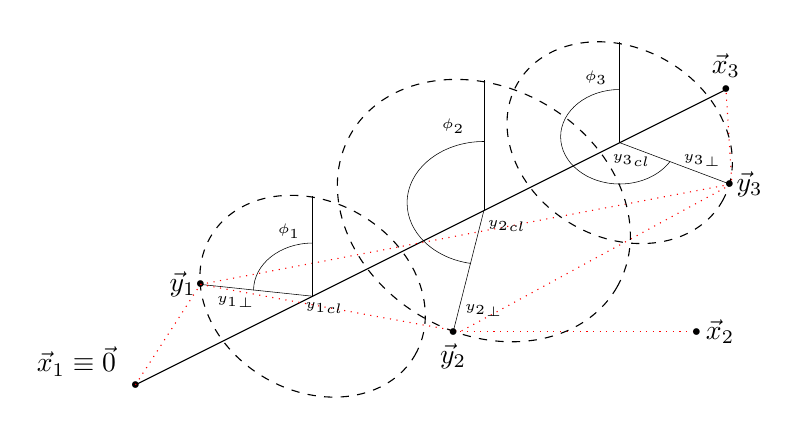
\begin{tikzpicture}[ scale=1.5]
\draw (0,0) node {\tiny$\bullet$} --(5,2.5) node {\tiny$\bullet$};
\draw (-0.5,0.2) node {$\vec{x}_1\equiv\vec{0}$};
\draw (5,2.7) node {$\vec{x}_3$};
   \draw [dashed] (1.5,0.75) circle [x radius=1cm, y radius=0.8cm, rotate=-30];
   \draw [very thin] (1.5,0.75)--(0.55,0.85);
     \draw  (0.55,0.85) node {\tiny$\bullet$};
          \draw  (0.4,0.85) node {$\vec{y}_1$};
      \draw [very thin] (1.5,1.2) arc (90:180:0.5cm and 0.4cm);
      \draw (1.3,1.3) node {\tiny$\phi_1$};
      \draw[dotted, color=red] (0,0)--(0.55,0.85) -- (2.75,0.45)--(5.05,1.7);
      \draw[dotted, color=red] (0.55,0.85) --(5.05,1.7)--(5,2.5);
       \draw[dotted, color=red] (2.75,0.45)--(4.75,0.45);
       \draw  (4.75,0.45) node {\tiny$\bullet$};
          \draw  (4.95,0.45) node {$\vec{x}_2$};
      \draw (0.85,0.7) node {\tiny${y_1}_\perp$};
      \draw (1.6,0.65) node {\tiny${y_1}_{cl}$};
   \draw [very thin] (1.5,0.75)--(1.5,1.6);
    \begin{scope}[shift={(+2.6,1.3)}]
       \draw [dashed] (1.5,0.75) circle [x radius=1cm, y radius=0.8cm, rotate=-30];
   \draw [very thin] (1.5,0.75)--(2.43,0.4);
     \draw  (2.43,0.4) node {\tiny$\bullet$};   
          \draw  (2.6,0.4) node {$\vec{y}_3$};   
     \draw [very thin] (1.5,0.75)--(1.5,1.6);
    \draw [very thin] (1.5,1.2) arc (90:328.5:0.5cm and 0.4cm);
          \draw (1.3,1.3) node {\tiny$\phi_3$};
      \draw (2.2,0.6) node {\tiny${y_3}_\perp$};
      \draw (1.6,0.6) node {\tiny${y_3}_{cl}$};
  \end{scope}
      \begin{scope}[shift={(+1,0.5)}, scale= 1.3]
      \draw (1.3,-0.04) node {\tiny$\bullet$};
      \draw (1.3,-0.2) node {$\vec{y}_2$};
       \draw [dashed] (1.5,0.75) circle [x radius=1cm, y radius=0.8cm, rotate=-30];
   \draw [very thin] (1.5,0.75)--(1.3,-0.04);
   \draw [very thin] (1.5,0.75)--(1.5,1.6);
    \draw [very thin] (1.5,1.2) arc (90:260:0.5cm and 0.4cm);
          \draw (1.3,1.3) node {\tiny$\phi_2$};
      \draw (1.5,0.1) node {\tiny${y_2}_\perp$};
      \draw (1.65,0.65) node {\tiny${y_2}_{cl}$};
  \end{scope}
\end{tikzpicture}
\caption{Coordinates chosen to analyze the collinear divergences in the first two terms in (\ref{jejejeje}). The ${y_i}_\perp$ measure the distance to the collinear line, ${\phi}_i$ represent the angles formed in the plane perpendicular to $\vec{x}_{3}$, and ${y_i}_{cl}$ the collinear separation from the origin. The red dotted line depicts the triangle diagram.}\label{frens}
\end{figure}

In this reference frame, the TOPT term in (\ref{jejejeje}) contributing to (\ref{assuca}) is proportional to
\begin{align}
I=&\int \prod_{i=1}^3\Big(d{y_i}_{cl} {y_i}_\perp d{y_i}_\perp d \phi_i\theta({y_i}_{cl})\Big)\prod_{j=1}^6\Big(\frac{1}{2|\vec{z_j}|+i\eta}\Big)\nonumber\times\\
&\times\frac{\theta({y_3}_{cl}-{y_1}_{cl})\theta({y_3}_{cl}-{y_2}_{cl})\theta({y_2}_{cl}-{y_1}_{cl})\theta({x_3}_{cl}-{y_3}_{cl})}{(-\Delta\tau_{31}+|\vec{z}_1|+|\vec{z}_3|+|\vec{z}_6|+i\eta) }\nonumber\\
&\times\frac{f(\{{y_i}_{cl}\},\{{y_i}_\perp\}, \{\phi_i\})}{(-\Delta\tau_{31}+|\vec{z}_1|+|\vec{z}_2|+|\vec{z}_4|+|\vec{z}_6|+i\eta)}\;,\label{guapo}
\end{align}
%:
where we introduce the $\theta$-functions to have the configuration in the middle diagram in Fig. \ref{fueraya2} and to avoid for now divergences arising from vertices going hard. $f(\{{y_i}_{cl}\},\{{y_i}_\perp\}, \{\phi_i\})$ is a finite function at the pinch surface containing all remaining terms for this contribution in (\ref{assuca}). It is easy to see that the intrinsic variables for the pinch surface are the $\{{y_i}_{cl}\}$, and the $\{{\phi_i}\}$. While the normal variables are the $\{{y_i}_{\perp}\}$. We have to study how the denominators in (\ref{guapo}) scale under the rescaling ${y_i}_{\perp}\to\lambda {y_i}_{\perp}$. For that we have that, assuming that we are in the region where the $\theta$-functions in (\ref{guapo}) are nonzero,
\begin{align}
\Delta\tau_{31}&=|\vec{x}_3|=|({x_3}_{cl}-{y_3}_{cl})^2+({y_3}_{cl}-{y_1}_{cl})^2+({y_1}_{cl})^2|^\frac{1}{2}\nonumber\\
&=|{x_3}_{cl}-{y_3}_{cl}|+|{y_3}_{cl}-{y_1}_{cl}|+|{y_1}_{cl}|
\end{align}
and that, taking all $\phi_i$ to be equal (since they are just intrinsic variables at the pinch surface),
\begin{align}
&|\vec{z}_1|+|\vec{z}_3|+|\vec{z}_6|=(({x_3}_{cl}-{y_3}_{cl})^2+\lambda^2({y_3}_\perp)^2)^\frac{1}{2}+\nonumber\\
&+(({y_1}_{cl})^2+\lambda^2({y_1}_\perp)^2)^\frac{1}{2}+(({y_3}_{cl}-{y_1}_{cl})^2+\lambda^2({y_3}_\perp-{y_1}_\perp)^2)^\frac{1}{2}\nonumber\\
&=({x_3}_{cl}-{y_3}_{cl})\Big(1+\frac{\lambda^2({y_3}_\perp)^2}{({x_3}_{cl}-{y_3}_{cl})^2}\Big)^\frac{1}{2}+{y_1}_{cl}\Big(1+\frac{\lambda^2({y_1}_\perp)^2}{({y_1}_{cl})^2}\Big)^\frac{1}{2}\nonumber\\
&+({y_3}_{cl}-{y_1}_{cl})\Big(1+\frac{\lambda^2({y_3}_\perp-{y_1}_\perp)^2}{({y_3}_{cl}-{y_1}_{cl})^2}\Big)^\frac{1}{2}\nonumber\\
&=({x_3}_{cl}-{y_3}_{cl})\Big(1+\frac{\lambda^2({y_3}_\perp)^2}{2({x_3}_{cl}-{y_3}_{cl})^2}+...\Big)+({y_3}_{cl}-{y_1}_{cl})\times\nonumber\\
&\times\Big(1+\frac{\lambda^2({y_3}_\perp-{y_1}_\perp)^2}{2({y_3}_{cl}-{y_1}_{cl})^2}+...\Big)+{y_1}_{cl}\Big(1+\frac{\lambda^2({y_1}_\perp)^2}{2({y_1}_{cl})^2}+...\Big)\;,
\end{align}
due to the $\theta$-functions in (\ref{guapo}). This calculation is similar for the other denominator. Having hence that in the collinear limit $\lambda\to0$ the TOPT propagators behave as
\begin{align}
&\frac{1}{(|\vec{z}_1|+|\vec{z}_3|+|\vec{z}_6|-\Delta\tau_{31}) (|\vec{z}_1|+|\vec{z}_2|+|\vec{z}_4|+|\vec{z}_6|-\Delta\tau_{31})}\nonumber\\
&\;\;\;\;\;\;\;\;\;\;\;\;\;\;\;\;\;\;\;\;\;\;\;\;\;\;\;\;\;\;\;\;\;\;\;\;\;\;\;{\sim}_{\lambda\to0}\;\frac{1}{\lambda^4}\;.
\end{align}
Note now that each volume element ${y_i}_\perp d {y_i}_\perp$ scales as $\lambda^2$ so that the integrand in (\ref{guapo}) scales as $\lambda^2$. Giving therefore no divergence whatsoever. Remember that in the Coleman-Norton picture, in the two collinear configurations, the vertices $\vec{y}_2$ and $\vec{y}_3$ migrated towards $\vec{y}_1$ respectively due to the shrinking of their respective lines. Let us discuss one of these cases next.\par
Note that in the integral encoding the collinear singularities (\ref{guapo}) we can safely take the limit ${y_2}_\perp\to{y_1}_\perp$, this can be done introducing a $\delta({y_2}_\perp^2-{y_1}_\perp^2)$ in this integral. Now we can take the collinear limit while the vertex $\vec{y}_2$ migrates to $\vec{y}_1$, as $({y_2}_{cl}-{y_1}_{cl},{y_1}_\perp,{y_3}_\perp)\to \lambda({y_2}_{cl}-{y_1}_{cl},{y_1}_\perp,{y_3}_\perp)$. This makes that the volume element in the normal variables scale as $\lambda^5$ while in the two TOPT propagators still give $\lambda^{-4}$ and the $1/2|\vec{z_2}|$ produces a $\lambda^{-1}$. Hence, we find that the collinear configuration predicted by the Coleman-Norton picture (where the line $\vec{z}_2$ shrinks) gives rise to a logarithmic divergence. This is precisely the same result we found in momentum-space in the first chapter.\par
For the other collinear divergence the treatment is the same. We see therefore how, in order to have a divergence, the Coleman-Norton configurations in Fig. \ref{fig:reddiag} (b)-(c) are necessary. However, we can not find a reason here why the diagram in Fig. \ref{fig:reddiag} (d) is excluded since the same divergence is present here. We could nonetheless have expected this since we are not making any difference between all the three external lines and we do not have anything that relates us to a picture where we can identify the external lines as final or initial on-shell states. It is possible that the last configuration gets excluded when using the LSZ formula in this context to take the external points as final (initial) on-shell states. This would require further investigation.\par

 The next term in (\ref{assuca}) has the same form as (\ref{jejejeje}) but with the substitution of $(\Delta\tau_{21},\Delta\tau_{23})\leftrightarrow(-\Delta\tau_{21},-\Delta\tau_{23})$. So that the configurations giving rise to divergences are the same as in Fig. \ref{fueraya} but with $\vec{x}_2$ all the way to the left, meaning that it has the smallest time compared to the other external vertices. The following four terms in (\ref{assuca}) have analogous configurations giving rise to divergences.\\
 

 
 We move on to analyze the first term in (\ref{assuca}) giving rise to an UV hard divergence, 
 \begin{align}
&\;\;\;\;\;\frac{1}{|\vec{z}_2|+|\vec{z}_3|+|\vec{z}_4|}\frac{1}{-\Delta\tau_{32}-|\vec{z}_4|+|\vec{z}_5|+|\vec{z}_6|}\times\nonumber\\
&\times\frac{2}{-2\Delta\tau_{31}+|\vec{z}_1|+|\vec{z}_6|+|\vec{z}_3|+|\vec{z}_1|+|\vec{z}_6|-|\vec{z}_2|-|\vec{z}_4|}\;.
\end{align}
The first denominator above encodes the hard divergence when $|\vec{z}_2|=|\vec{z}_3|=|\vec{z}_4|=0$. In this case the other two terms give additional divergences whenever the three external vertices lie in the same line with $x_3$ having the largest time. The second term gives a divergence for the collinear ordering $\vec{y}_2$-$\vec{x}_2$-$\vec{y}_3$-$\vec{x}_3$ 
 \begin{figure}[ht!]
\centering
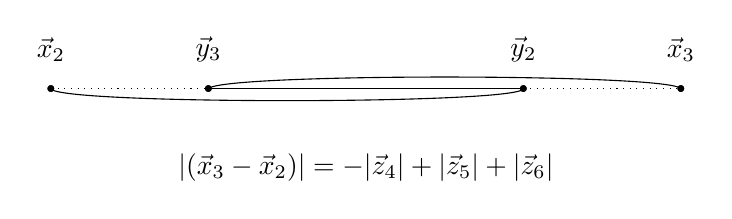
\begin{tikzpicture}
\draw (2,0) node {\tiny$\bullet$} -- (6,0) node {\tiny$\bullet$};
\draw (0,0)node {\tiny$\bullet$};
\draw (8,0) node {\tiny$\bullet$};
\draw[dotted,thin] (0,0)node {\tiny$\bullet$} -- (2,0) node {\tiny$\bullet$};
\draw[dotted,thin] (6,0)node {\tiny$\bullet$} -- (8,0) node {\tiny$\bullet$};
\draw (0,0.5)node {$\vec{x}_2$};
\draw (8,0.5)node {$\vec{x}_3$};
\draw (2,0.5)node {$\vec{y}_3$};
\draw (6,0.5)node {$\vec{y}_2$};
\draw (4,-1)node {$|(\vec{x}_{3}-\vec{x}_2)|=-|\vec{z}_4|+|\vec{z}_5|+|\vec{z}_6|$};
\draw (0,0) .. controls (.1,-0.2) and (5.9,-.2) .. (6,0);
\draw (2,0) .. controls (2.1,0.2) and (7.9,.2) .. (8,0);
\end{tikzpicture}
\end{figure}

The third term cannot give rise to a divergence since the first term in its denominator requires the collinear ordering $\vec{x}_1$-$\vec{y}_1$-$\vec{y}_3$-$\vec{x}_3$ while the second requires $\vec{x}_1$-$\vec{y}_3$-$\vec{y}_2$-$\vec{y}_1$-$\vec{x}_3$. All the remaining hard terms have analogous divergences. The terms with opposite time differences are the same as those already discussed but the time ordering of the external vertices must be read from right to left. From power counting it is possible to show that in the hard limit $(|\vec{z}_1|,|\vec{z}_2|,|\vec{z}_3|)\to\lambda(|\vec{z}_1|,|\vec{z}_2|,|\vec{z}_3|)$ the integral scales as $\lambda^2$ (avoiding the zeroth order lightcone singularity when $\Delta\tau_{32}=|\vec{z}_5|+|\vec{z}_6|$) so that no hard divergence is present. This is the same scaling that one can derive from the momentum-space diagram. \par

 We have therefore seen that our newly developed coordinate-space TOPT description for the scalar cubic theory offers a very neat causality and space configuration picture, predicting the same degree of divergence as in the momentum-space picture for Coleman-Norton-like configurations. As we will see next, these results are easily generalizable to gauge theories such as QED since we will have the same topologies in our diagrams. We will apply these results to the one-loop electromagnetic form factor.
 
 \subsection{Quark electromagnetic form factor in coordinate-space TOPT}
 Let us now extend our treatment of TOPT to fermions. We have to recover the expression of an arbitrary Green's function in (\ref{dadada441}) but distinguishing now between fermion and scalar (these will be vectors in QED) lines. The fermion lines will require special treatment, we have to study the expression
 \begin{align}
 I^\mu_j&=\int dz^0_{j}\frac{z_j^\mu\delta(z_{j}^0-\epsilon_{jk}y_k^0-\epsilon'_{jc}x^0_c)}{(-{z_{j}^0}^2+{\vec{z}_j}^{\;2}+i\eta)^2}\nonumber\\
 &=\int_{-\infty}^{+\infty}\frac{dE^0_j}{2\pi}\int dz^0_{j}\frac{z_j^\mu e^{iE^0_j(z_{j}^0-\epsilon_{jk}y^0_k-\epsilon'_{jc}x^0_c)}}{(-{z_{j}^0}^2+{\vec{z}_j}^{\;2}+i\eta)^2}\;.
\end{align}
Now we use the Cauchy's integral theorem to carry out the integral in $z_j^0$ obtaining
 \begin{align}
 I^\mu_j&=\frac{i\hat{z}_j^\mu}{(2|\vec{z}_j|+i\eta)^3}\Big(2\hat{z}_j^0\frac{\partial}{\partial \hat{z}_j^0}-2\sum_{i=1}^3\delta^{\mu i}\Big)\int_{-\infty}^{+\infty}\frac{dE^0_j}{2\pi}\nonumber\times\\
& \times \Big(\theta (E^0_j)e^{-iE_j^0(\epsilon_{jk}y^0_k+\epsilon'_{jc}x^0_c-|\vec{z}_j|-i\eta)}+\nonumber\\
&\;\;\;\;\;\;\;\;\;\;+\theta (-E^0_j)e^{-iE_j^0(\epsilon_{jk}y^0_k+\epsilon'_{jc}x^0_c+|\vec{z}_j|+i\eta)}\Big) \;,
\end{align}
where we have defined the lightlike vector $\hat{z}_j^\mu=(|\vec{z}_j|,\vec{z}_j)$ (see Appendix C for the details of this calculation). With this representation of the fermion propagator we can use all results obtained in coordinate-space TOPT to all orders including fermion lines. These will only add the term in big brackets in the first line, which do not depend on $y_0$, so that the delta functions of conservation of energy are still obtained in the same way as in (\ref{dadada444}).\par


\begin{figure}[ht!]
\centering
\begin{tikzpicture}
\begin{feynman}
\vertex (a);
\vertex [left=0cm of b] (ktt);
\vertex [right=1.08cm of ktt] (ktthh){\tiny$\bullet$};
\vertex [above=0.3cm of ktthh] (ktth2h){$x_1$};
\vertex [right=1.3 cm of a] (b);
\vertex [above=0.01 cm of b] (11){$y_1$};
\vertex [right=0.1cm of b] (H){$\gamma^\mu$};
\vertex [right=3.5cm of b] (Hh){$\equiv-ie\,\Gamma_{(1)}^\mu(x_1,x_2,x_3)$};
\vertex [right=4.5cm of Hh] (Hha);
\vertex [above right=1.4cm of b] (k);
\vertex [above right=1.14cm of b] (kjj){\tiny$\bullet$};
\vertex [above right=2.15 cm of b] (kjj){\tiny$\bullet$};
\vertex [right=0.5cm of kjj] (kjdj){$x_2$};
\vertex [above=0.01cm of k] (kkkk){$y_2$};
\vertex [above right=1cm of k] (t);
\vertex [below right=1.4 cm of b] (f1);
\vertex [below right=1.14 cm of b] (f111){\tiny$\bullet$};
\vertex [above left=1.35 cm of f111] (f1121){\tiny$\bullet$};
\vertex [below right=2.15 cm of b] (kjj1){\tiny$\bullet$};
\vertex [right=0.5cm of kjj1] (kjdj1){$x_3$};
\vertex [below=0.01cm of f1] (kkkk){$y_2$};
\vertex [below right=1cm of f1] (c);

\diagram* {
(a) -- [photon,edge label=1] (b)  (k)-- [gluon, edge label=4] (f1)
(b)-- [] (k)
(k)-- [fermion] (b)
(b)-- [edge label=3] (k)
(k)-- [] (t)
(t)-- [fermion,edge label=6] (k)
(f1)-- [fermion,edge label=5] (c)
(c)-- [] (f1)
(f1) -- [] (b)
(b) -- [fermion] (f1)
(f1) -- [edge label=2] (b)

};
\end{feynman}
\end{tikzpicture}
\caption{One loop contribution to the quark EM vertex function in equation in coordinate-space. The numbers refer to the labeling of the displacement vectors $\vec{z}_j$.}\label{alohababe}
\end{figure}
Let us apply this result to the one-loop quark electromagnetic form factor in Fig. \ref{alohababe}. We can readily see that, remembering the minus sign from the fermion loop,
\begin{align}
 \Gamma_{(1)}^\mu&(x_1,x_2,x_3)=\frac{g^2C_F}{(2\pi)^9}\int\prod_{i=1}^3d^3y_i\Big(\prod_{j=1,4}\frac{1}{2|\vec{z_j}|+i\eta}\Big)\times\nonumber\\
 &\times\Big(\prod_{l\neq1,4}\frac{\hat{z}_l^{\mu_l}}{(2|\vec{z}_l|+i\eta)^3}\Big(2\hat{z}_l^0\frac{\partial}{\partial \hat{z}_l^0}-2\sum_{i=1}^3\delta^{\mu_l i}\Big)\Big)\times \nonumber\\
 &\times \gamma_{\mu_6}\gamma_\nu\gamma_{\mu_3}\gamma^\mu\gamma_{\mu_2}\gamma^\nu\gamma_{\mu_5}\varUpsilon_S(\{y_i\})\,,
 \end{align}
 where $\varUpsilon_S(\{y_i\})$ was defined in (\ref{heil}) and contains the TOPT propagators calculated in (\ref{assuca}).\par
 It is very interesting to see now how the hard logarithmic singularity that we expect from the momentum-space picture arises in our coordinate-space diagram. Recall that in the scalar case, under the rescaling $(|\vec{z}_1|,|\vec{z}_2|,|\vec{z}_3|)\to\lambda(|\vec{z}_1|,|\vec{z}_2|,|\vec{z}_3|)$, the integrands containing the hard singularities in (\ref{assuca}) scaled as $\lambda^2$. Now two of the lines that shrink, $|\vec{z}_2|$ and $|\vec{z}_3|$, are fermion lines and each produce a factor of $\lambda^{-1}$ extra with respect to the scalar case. Giving therefore a scaling of $\lambda^0$ corresponding to the logarithmic singularity we expect from power counting in the momentum-space description. In collinear cases the scaling goes along as in the scalar case, giving a logarithmic divergence strictly linked with the Coleman-Norton picture. However the same problem as in the scalar case arises: the diagrams in Fig. \ref{fig:reddiag} (d) are not excluded to give a divergence. As in the scalar case, here we should make a connection between external points and on-shell final or initial states through an adapted version of the LSZ formula. Summing up, our newly developed TOPT treatment is in agreement with the Coleman-Norton picture but some further investigation is required to get a full answer that excludes the non-Coleman-Norton cases. Also, the interpretation of soft lines becomes not always apparent in the coordinate-space TOPT treatment.
 \section{Overview}
In this paper we have discussed the results of factorization of QCD amplitudes and studied in particular the one-loop contribution to the jet function in coordinate space, finding that the most divergent part of it is proportional to a fermion propagator. This may be though as a configuration where the gluon emerging from the cusp of the Wilson line travels collinear with the fermion to the external point, producing hence the divergence. LSZ reduction of our result shows that we recover the correct divergence expected from the momentum space previous known results. We computed also a radiated contribution to the jet-function although no clear result is found here. Seeking further interpretations of the Feynman parameters and more intuition on collinear configurations we presented TOPT in momentum space, where lines could be seen as on-shell but no there was no conservation of energy at the vertices, and the Feynman parameter could be identified as the ratio of the particle's flying time and on-shell energy. All these facts are in deep connection with the Coleman-Norton picture. Finally, coordinate-space TOPT helped us to indeed find Coleman-Norton-like spatial collinear configurations of vertices as a condition for divergencies in the amplitudes. I believe that a careful analysis of which configurations give or not imaginary parts to the amplitudes and their connection to Causality and Unitarity may be much more enlightening than the present paper, which is just the starting point to do so. \\


\section{Aknowledgments}

I want to thank professor Eric Laenen for his guidance and interesting remarks and the whole NIKHEF staff for creating such a welcoming atmosphere. Also express my gratefulness to the Amsterdam Science Talent Scholarship for allowing me to stay abroad and to the Spanish Grant MINECO:FPA2016-75654-C2-1-P as well as the IPARCOS institute.




\section{Appendices}
\subsection{Factors in the one-loop radiated jet function contribution}
Here we present the factors that appear in (\ref{HAHAHA}):

\begin{align}
M^2=m^2-(\square+(1-\alpha_5 n))^2\alpha^{-2}
\end{align}

\begin{align}
B^\mu&=(\slashed\square\alpha^{-1}+\slashed y)\Big[\slashed n\Big((1-\alpha_2)\slashed x-\alpha_1\alpha_2\alpha^{-1}\slashed\square\Big)\gamma^\mu\times\nonumber\\
&\times\Big((1-\alpha_2)\slashed x-\alpha_1\alpha_2\alpha^{-1}(\slashed\square+(1-\alpha_5)\slashed n)\Big)-\nonumber\\
&-\alpha_2\slashed n \gamma^\mu\Big(\alpha_1(1-\alpha_1\alpha_2)(\square+(1-\alpha_5) n))^2+\nonumber\\
&+(1-\alpha_2)x^2+2\alpha_1(1-\alpha_2)x\cdot(\square+(1-\alpha_5) n))\Big)\Big]+\nonumber\\
&+\alpha^{-1}\Big((\square+(1-\alpha_5)n)^2\slashed n+\slashed y\slashed n\slashed\square\Big)\gamma^\mu\times\nonumber\\
&\times\Big((1-\alpha_2)\slashed x-\alpha^{-1}\big(\slashed\square+(1-\alpha_5) \slashed n)\big)\Big)
\end{align}

\begin{align}
&A_{\rho\nu}^\mu=- \alpha_1\alpha_2+\times\nonumber\\
&\times\Big(\alpha^{-2}(1-\alpha_1\alpha_2)(2(\square+(1-\alpha_5)n)_\nu)+2\alpha^{-1}(1-\alpha_2)\slashed n\Big)\gamma_\rho\slashed n\gamma^\mu+\nonumber\\
&+(\slashed\square\alpha^{-1}+\slashed y)\Big(\alpha_1\alpha_2(1-\alpha_1\alpha_2)\slashed n \gamma^\mu g_{\rho\nu}+\slashed n(\alpha_1\alpha_2)^2\alpha^{-1}\gamma_\rho\gamma^\mu\gamma_\nu\Big)-\nonumber\\
&-\gamma_\rho\slashed n\Big(\alpha_1\alpha_2\alpha^{-1}\gamma_\nu\gamma^\mu\big((1-\alpha_2)\slashed x-\alpha_1\alpha_2\alpha^{-1}(\slashed\square+(1-\alpha_5)\slashed n)\big)\nonumber\\
&+\big((1-\alpha_2)\slashed x-\alpha_1\alpha_2\alpha^{-1}\slashed\square\big)\gamma^\mu(\alpha_1\alpha_2\alpha^{-1}\gamma_\nu)\Big)-\nonumber\\
&-\alpha^{-1}g_{\rho\nu}\slashed n\gamma^\mu\Big((1-\alpha_2)\slashed x-\alpha_1\alpha_2\alpha^{-1}(\slashed\square+(1-\alpha_5)\slashed n)\Big)+\nonumber\\
&+\alpha_1\alpha_2\Big(2\alpha^{-2}(\square+(1-\alpha_5) n)_\rho\slashed n+\alpha^{-1}\slashed y\slashed n\gamma_\rho\Big)\gamma^\mu\gamma_\nu
\end{align}

\subsection{Unitarity and cut diagrams in TOPT}

The unitarity of the $S$ matrix has a fundamental importance since it implies the conservation of probability in the field theory. This matrix is related to measurable on-shell scattering amplitudes (the matrix $T$) that are in turn associated to general Green's functions, $G$, through reduction formulas. 
Following \cite{QFTSterman} we will now employ time ordered perturbation theory in momentum-space to prove the unitarity of the scattering matrix $S$ for a non-gauged theory which, remembering the relation with the transition matrix $T$, $S\equiv \mathbb{I}+iT$, implies,
\begin{equation}
i(T-T^\dagger)=-T^\dagger T\;.\label{Tmat}
\end{equation}

Take now a general sum of TO diagrams, $G$,
\begin{align}
&G(p_1,...,p_m;k_1,...,k_n)=i\sum_{\substack{\text{TO of $G$} \\ \tau}}\prod_{loops\;i}\int\frac{d^3\vec{l}_i}{(2\pi)^3}\nonumber\\
&\times\prod_{int.\;lines\;j}\frac{N_G(\{p\},\{l_i\})}{2\omega_j(\{l_i\},\{p\})}\prod_{states\,a}\frac{1}{E_a-S_a+i\eta}\label{kinoto}\;,
\end{align}
where we have introduced an extra $i$ so that if its truncated according to the usual reduction formula, it contributes to the $T$ matrix. $N_G$ contains all numerator factors and also the total energy conservation delta function, $-(2\pi)\delta(E_{in}-E_{out})$.
\begin{figure}[ht!]
\centering
\begin{tikzpicture}
\begin{feynman}
\vertex (a){$k_1$};
\vertex [below right=1.45 cm of a] (b);
\vertex [below=1.55 cm of a] (h){.};
\vertex [below=.2 cm of h] (hh){.};
\vertex [below=.2 cm of hh] (hhh){.};
\vertex [right=1.2 cm of b] (c);
\vertex [above right=1 cm of c] (c3){$p_1$};
\vertex [below=1.5 cm of c3] (f){.};
\vertex [below=.2 cm of f] (ff){.};
\vertex [below=.2 cm of ff] (fff){.};
\vertex [below=1.4 cm of b] (b1);
\vertex [below=0.4 cm of b] (e1){$L_\gamma$};
\vertex [below=1.4 cm of c] (c1);
\vertex [below=0.4 cm of c] (e2){$R_\gamma$};
\vertex [below left=0.8 cm of b1] (b2){$k_n$};
\vertex [below right=0.8 cm of c1] (c2){$p_m$};

\vertex [left=0.1cm of b] (kk);
\vertex [left=0.1cm of b1] (kk1);
\vertex [below right=1cm of kk1] (kk2){$\gamma$};


\diagram* {
(a)--(b)
(c)--(c3)
(b)--[half right,looseness=1.7](b1)
(b1)--[half right,looseness=0](c1)
(b)--[half left,looseness=0](c)
(c)--[half left,looseness=1.7](c1)
(b1)--(b2)
(c1)--(c2)

};\draw[dashed] 
  ([yshift=18pt]$ (s)!1.5!(kk) $ ) -- 
  ([yshift=-20pt]$ (s)!1.5!(kk1) $ );
\end{feynman}
\end{tikzpicture}
\caption{General cut diagram $G_\gamma$ of equation (\ref{joretio}).}\label{kaka}
\end{figure}
We will denote a cut graph by $G_\gamma$ obtained from cutting internal lines, i.e. choosing the internal cut lines as final states, with cut $\gamma$ from the overall graph $G$ (see Fig. \ref{kaka}). The cut $\gamma$ is basically replacing the TO ``propagator'' $(E_\gamma-S_\gamma+i\eta)^{-1}$ by $-2\pi i \delta(E_\gamma-S_\gamma)$, i.e. taking the discontinuity of it. Here $S_\gamma=\sum_{m=1}^{n_\gamma}\omega_m$ is the sum of energies of the final states in the cut $\gamma$. $L_\gamma$ and $R_\gamma$ are the subgraphs to the left and right of $\gamma$ and the momentum flow is from left to right. Note that the time orderings of $G_\gamma$ are the same as the time orderings of $G$ and that the denominators in the right part $R_\gamma$ have to be complex conjugated. In this way we have

\begin{align}
G_\gamma&(\{p_j\},\{k_i\})\equiv\sum_{\substack{\text{TO of $G_\gamma$} \\ \tau}}\int\prod_{\substack{\text{loops of $G$} \\ l}}\frac{d^3\vec{q}_l}{(2\pi)^3}\prod_{\substack{\text{int. lines} \\ b}}\frac{N_{G}(\{q_l\})}{2\omega_b}\times\nonumber\\
&\times \prod_{\substack{\text{states in $R$} \\ s}}\Big(E_s-S_s-i\eta\Big)^{-1}(2\pi)\delta(E_\gamma-\sum_k^{n_\gamma}\omega_k)\times\nonumber\\
&\times\prod_{\substack{\text{states in $L$} \\ s'}}\Big(E_{s'}-S_{s'}+i\eta\Big)^{-1}\;.\label{joretio}
\end{align}
%This general cut diagram contributing to (\ref{kinoto}) can be expressed as
%\begin{align}
%G_\gamma(\{p_j\},\{k_i\})&=s_\gamma^{-1}\Big(\prod_{\substack{\text{final-st.  lines} \\ k}}\int\frac{d^3\vec{l}_k}{(2\pi)^3 2\omega(\vec{l}_k)}\Big)(2\pi)^3\delta^{(3)}\Big(\sum_i \vec{k}_i-\sum_k \vec{l}_k\Big)\times\nonumber\\
%&\times R_\gamma^\ast(\{p_j\},\{l_k\})2\pi\delta\Big(\sum_ik_i^0-\sum_k l_k^0\Big)L_\gamma(\{l_k\},\{k_i\})\;,\label{fueros}
%\end{align}
%where $s_\gamma^{-1}$ represents a symmetry factor associated with having identical bosons in the final states produced by $\gamma$. Now we will use TOPT to evaluate $L_\gamma$ and $R_\gamma$. Remembering equation (\ref{TOdiag}) these are
%\begin{align}
%L_\gamma(\{l_k\},\{k_i\})&=-\sum_{\substack{\text{TO\;contrib.} \\ \tau}}\int\prod_{\substack{\text{loops in $L$} \\ l}}\frac{d^3\vec{q}_l}{(2\pi)^3}\times\nonumber\\
%&\times\prod_{\substack{\text{int. lines} \\ b}}\frac{N_{L_\gamma}(\{k_i\},\{l_k\},\{q_l\})}{2\omega_b}\prod_{\text{states\,$a$\,of\, $\tau$}}\frac{1}{E_a-S_a+i\eta}\nonumber\\
%\,\\
%R_\gamma(\{p_j\},\{l_k\})&=-\sum_{\substack{\text{TO\;contrib.} \\ \tau}}\int\prod_{\substack{\text{loops in $L$} \\ l}}\frac{d^3\vec{q}_l}{(2\pi)^3}\times\nonumber\\
%&\times\prod_{\substack{\text{int. lines} \\ b}}\frac{N_{R_\gamma}(\{p_j\},\{l_k\},\{q_l\})}{2\omega_b}\prod_{\text{states\,$a$\,of\, $\tau$}}\frac{1}{E_a-S_a+i\eta}\nonumber\,.
%\end{align}
%Here $N_{L_\gamma}$ and $N_{R_\gamma}$ include all numerator factors for TOPT and group and symmetry factors as well as fermionic signs. Using now the spatial momenta conservation delta function in eq. (\ref{fueros}) and noting that the loops of the full graph $G$ can be thought as the union of the loops of $L_\gamma$ and $R_\gamma$, along with any $n_\gamma-1$ of the final state momenta \cite{QFTSterman}, where $n_\gamma$ is the number of lines in the final state $\gamma$, we obtain

%Turns out that the numerator and symmetry factor $N_G=s_\gamma^{-1}N_{R_\gamma}N_{L_\gamma}$ does not depend on the cut $\gamma$ and its the same as the overall diagram $G$. This proof is presented in \cite{QFTSterman}.\par
Now we will sum over all the possible cuts $\gamma$ of the diagram $G$. To do so remember the distribution identity 
\begin{equation}
(x+i\eta)^{-1}-(x-i\eta)^{-1}=-2\pi i\delta(x)\;,
\end{equation}
and use it into (\ref{joretio}) interchanging the sum over final states and time orders of $G_\gamma$ to get
\begin{align}
&\sum_{\gamma} G_\gamma(\{p_j\},\{k_i\})=\sum_{\substack{\text{orders of $G_\gamma$} \\ \tau}}\int\prod_{\substack{\text{loops of $G$} \\ l}}\frac{d^3\vec{q}_l}{(2\pi)^3}\prod_{\substack{\text{int. lines of $G$} \\ b}}\nonumber\\
&\times\frac{N_{G}(\{q_l\})}{2\omega_b}\sum_{\substack{\text{final states of  $\tau$} \\ \gamma}}\Big\{\prod_{\substack{\text{states of $R_\gamma$} \\ s}}\Big(E_s-S_s-i\eta\Big)^{-1}\nonumber\times\\
&\times\prod_{\substack{\text{states of $L_\gamma$} \\ s'}}\Big(E_{s'}-S_{s'}+i\eta\Big)^{-1}\nonumber\times\\
&\times i\Big[\Big(E_\gamma-S_\gamma+i\eta\Big)^{-1}-\Big(E_\gamma-S_\gamma-i\eta\Big)^{-1}\Big]\Big\}\;.\label{houlot}
\end{align}

Let's prove unitarity using induction, consider the $A$ cuts of a diagram $G$ with $A+1$ vertices and the integrand in (\ref{houlot}) for a fixed time ordering of $G_\gamma$. Remember that the cut $\gamma$ separates the left part $L_\gamma$ with states from 1 to $\gamma-1$, and the right part with states from $\gamma+1$ to $A$. Assume now that the relation
\begin{align}
&\sum_{\gamma=1}^A \prod_{j=\gamma+1}^A(E_j-S_j-i\eta)^{-1}\prod_{i=1}^{\gamma-1}(E_i-S_i+i\eta)^{-1}\times\nonumber\\
&\times\Big[(E_\gamma-S_\gamma+i\eta)^{-1}-(E_\gamma-S_\gamma-i\eta)^{-1}\Big]\nonumber\\
&=\Big[\prod_{j=1}^A(E_j-S_j+i\eta)^{-1}-\prod_{j=1}^A(E_j-S_j-i\eta)^{-1}\Big]\label{unit}
\end{align}
holds (here, if the starting index of the product or the sum is bigger that the ending index we suppose there is no product). Defining $(\pm i\eta_j)\equiv(E_j-S_j\pm i\eta)$, let us prove that holds for three vertices, i.e. $A=2$. Equation (\ref{unit}) in this case amounts to
\begin{align}
\sum_{\gamma=1}^2 \prod_{j=\gamma+1}^2&(-i\eta_j)^{-1}\Big[(+i\eta_\gamma)^{-1}-(-i\eta_\gamma)^{-1}\Big]\prod_{i=1}^{\gamma-1}(+i\eta_i)^{-1}=\nonumber\\
&=(-i\eta_2)^{-1}\Big((+i\eta_1)^{-1}-(-i\eta_1)^{-1}\Big)+\nonumber\\
&\;\;\;+\Big((+i\eta_2)^{-1}-(-i\eta_2)^{-1}\Big)(+i\eta_1)^{-1}\nonumber\\
&=(+i\eta_1)^{-1}(+i\eta_2)^{-1}-(-i\eta_1)^{-1}(-i\eta_2)^{-1}\,.
\end{align}

Now we move on to prove this relation for a diagram with $A+2$ vertices supposing it holds for $A+1$ vertices,
\begin{align}
&\sum_{\gamma=1}^{A+1} \prod_{j=m+1}^{A+1}(-i\eta_j)^{-1}\Big[(i\eta_\gamma)^{-1}-(-i\eta_\gamma)^{-1}\Big]\prod_{i=1}^{\gamma-1}(+i\eta_i)^{-1}=\times\nonumber\\
&=(-i\eta_{A+1})^{-1}\sum_{m=1}^A\Big\{\prod_{j=\gamma+1}^A(-i\eta_j)^{-1}\Big[(i\eta_\gamma)^{-1}-(-i\eta_\gamma)^{-1}\Big]\times\nonumber\\
&\;\;\;\times\prod_{i=1}^{\gamma-1}(+i\eta_i)^{-1}+\Big[(i\eta_{A+1})^{-1}-(-i\eta_{A+1})^{-1}\Big]\prod_{i=1}^{A}(i\eta_i)^{-1}\nonumber\\
&\stackrel{(\ref{unit})}{=}(-i\eta_{A+1})^{-1}\Big[\prod_{j=1}^A\Big((i\eta_j)^{-1}-(-i\eta_j)^{-1}\Big)\Big]+\nonumber\\
&\;\;\;+\Big[(i\eta_{A+1})^{-1}-(-i\eta_{A+1})^{-1}\Big]\prod_{i=1}^{A}(i\eta_i)^{-1}=\nonumber\\
&=\Big[\prod_{j=1}^{A+1}(i\eta_j)^{-1}-\prod_{j=1}^{A+1}(-i\eta_j)^{-1}\Big]\;,
\end{align}
so that the proof of equation (\ref{unit}) is complete. Using this into (\ref{houlot}) we obtain
\begin{align}
&\sum_{\gamma} G_\gamma(\{p_j\},\{k_i\})=\sum_{\substack{\text{orders of $G_\gamma$} \\ \tau}}\int\prod_{\substack{\text{loops of $G$} \\ l}}\frac{d^3\vec{q}_l}{(2\pi)^3}\times\nonumber\\
& \times\prod_{\substack{\text{int. lines of $G$} \\ b}}\frac{N_{G}(\{p_j\},\{k_i\},\{q_l\})}{2\omega_b}\times\nonumber\\
&\times i\Big[\prod_{\substack{\text{states of $G$} \\ s}}(E_s-S_s+i\eta)^{-1}-\prod_{\substack{\text{states of $G$} \\ s}}(E_s-S_s-i\eta)^{-1}\Big]
\end{align}
and hence to the well known unitarity relation
\begin{equation}
\sum_{\gamma} G_\gamma(\{p_j\},\{k_i\})=2\text{Im} \,G(\{p_j\},\{k_i\})\;.\label{Unitarity}
\end{equation}
This equation is the graphical representation of (\ref{Tmat}). Nevertheless, it is much more general since it does not require the external lines of the cut graph to be on the mass shell.\par
All things said, this proof of unitarity, although general, does not include gauge theories. It assumes that all propagator poles correspond to physical states so that (\ref{Unitarity}) is an equation for the physical $S$ matrix. However, since in gauge theories unphysical degrees of freedom (unphysical polarizations or ghosts) propagate, these can appear in the final states of the cut. Hence our proof does not apply for these theories. The proof of unitarity for QED and QCD can be found in \cite{QFTSterman}, it relies on the use of Ward identities to show that the sum over physical polarizations equals the sum over gauge polarizations.
\subsection{TOPT propagators for fermions}
In the TOPT treatment in coordinate-space we needed to carry out the $z^0_j$ integrations for each line after introducing the unity in form of an integration in the auxiliary energy $E_j$ and a delta function $\delta(z_j^0-\epsilon_{jk} y_k^0-\epsilon'_{jc}x_c^0)$. The contribution from fermion lines will be proportional to the integral
 \begin{align}
 I^\mu_j&=\int dz^0_{j}\frac{z_j^\mu\delta(z_{j}^0-\epsilon_{jk}y_k^0-\epsilon'_{jc}x^0_c)}{(-{z_{j}^0}^2+{\vec{z}_j}^{\;2}+i\eta)^2}\nonumber\\
 &=\int_{-\infty}^{+\infty}\frac{dE^0_j}{2\pi}\int dz^0_{j}\frac{z_j^\mu e^{iE^0_j(z_{j}^0-\epsilon_{jk}y^0_k-\epsilon'_{jc}x^0_c)}}{(-{z_{j}^0}+{\vec{z}_j}+i\eta)^2({z_{j}^0}+{\vec{z}_j}+i\eta)^2}\;.
\end{align}
We see that the integrations in the $z_j^0$ will pick up, after proper closing of the contour of integration, the residues of the two double poles $z_j^0=\pm(|\vec{z}_j|+i\eta)$. These are:
\begin{itemize}
\item For spatial components of the numerator the integrand $f$ has residues
\begin{align}
&\text{Res}(f,\pm(|\vec{z}_j|+i\eta))=\nonumber\\
&=\theta(\pm E_j)z_j^i\Big(\frac{iE_j(2|\vec{z}_j|+2i\eta)\mp2}{(2|\vec{z}_j|+2i\eta)^3}\Big)e^{\pm iE_j(|\vec{z}_j|\mp\epsilon_{jk}y_k^0\mp\epsilon'_{jc}x^0_c)}
\end{align}
\item For the time component of the numerator 
\begin{align}
&\text{Res}(f,\pm(|\vec{z}_j|+i\eta))=\nonumber\\
&=\theta(\pm E_j)|\vec{z}_j|\Big(\frac{iE_j(2|\vec{z}_j|+2i\eta)}{(2|\vec{z}_j|+2i\eta)^3}\Big)e^{\pm iE_j(|\vec{z}_j|\mp\epsilon_{jk}y_k^0\mp\epsilon'_{jc}x^0_c)}\;.
\end{align}
\end{itemize}
In this way, taking into account the sign of the orientation for the contour integrals and dropping $i\eta$s in numerators and after defining the lightlike vector $\hat{z}^\mu=(|\vec{z}_j|,\vec{z}_j)$,
this becomes, 
 \begin{align}
 I^\mu_j&=\frac{i\hat{z}_j^\mu}{(2|\vec{z}_j|+i\eta)^3}\Big(2\hat{z}_j^0\frac{\partial}{\partial \hat{z}_j^0}-2\sum_{i=1}^3\delta^{\mu i}\Big)\nonumber\times\\
& \times\int_{-\infty}^{+\infty}\frac{dE^0_j}{2\pi} \Big({\theta (E^0_j)e^{-iE_j^0\alpha_j^-}+\theta (-E^0_j)e^{-iE_j^0\alpha_j^+}}\Big) \;.
\end{align}
This expression is ready to employ all the know results of scalar TOPT in coordinate-space.




%-------------------------------------------------------------------------------------------------------
\begin{thebibliography}{21}
\bibitem{Bonoc}
D. Bonocore, E. Laenen, \textit{A factorization approach to next-to-leading-power threshold logarithms}, et al. J. High Energ. Phys. (2015).
 \bibitem{Tod}
I.T. Todorov, \textit{Analytic Properties of Feynman Diagrams in Quantum Field Theory}. International Series of Monographs in Natural Philosophy Volume 38, Pergamon Press (1971).
 
\bibitem{ColNor}
S. Coleman and R.E. Norton \textit{Singularities in the physical region}. N. Cim. 38 438-442 (1965).
\bibitem{ACME}
W. C. Campbell et al., \textit{Advanced cold molecule electron EDM}, 	
EPJ Web of Conferences, Volume 57, https://doi.org/10.1051/epjconf/20135702004, (2013).
\bibitem{QFTSterman}
G. Sterman, \textit{An Introduction to Quantum Field Theory}. Cambridge University Press (1993).
\bibitem{Sterman1}
G. Sterman, \textit{Mass divergences in annihilation processes. I. Origin and nature of divergences in cut vacuum polarization diagrams}. Phys. Rev. D, v- 17 n. 10, 2773-2788 (1977).
\bibitem{RicBon}
D. Bonocore, E. Laenen et al., \textit{A factorization approach to next-to-leading-power threshold logarithms}.  arXiv:1503.05156v2 (2015).
\bibitem{Collins}
J.C. Collins, \textit{Sudakov Form Factors}. Adv.Ser.Direct.High Energy Phys., 573-614, (2003).
\bibitem{Stermannotes}
G. Sterman, \textit{Partons, Factorization and Resummation}. TASI 95 (1996).
\bibitem{Nakahara}
M. Nakahara, \textit{Topology, Geometry and Physics}.  Graduate Student Series in Physics (2003).
\bibitem{DGM}
L.J. Dixon, E. Gardi, L. Magnea, \textit{On soft singularities at three loops and beyond}. High Energ. Phys. (2011).
\bibitem{CFR}
S. Catani, D. de Florian, and G. Rodrigo, \textit{Space-like (versus time-like) collinear limits in QCD: Is factorization violated?}.  High Energ. Phys. (2012).	arXiv:1112.4405.
\bibitem{FSS}
J. R. Forshaw, M.H. Seymour, and A. Siodmok, \textit{On the breaking of collinear factorization in QCD.}  High Energ. Phys. (2012). arXiv:1206.6363.
\bibitem{ErdoganCS}
O. Erdogan, \textit{Coordinate-space singularities of massless gauge theories}.  P. Rev. D \textbf{89} (2014).
\bibitem{jeronero}
G. Korchemsky and A. Radyushkin,   Nucl. Phys. \textbf{B283}, 342-364 (1987).
\bibitem{Martinus}
M. Veltman, \textit{Diagrammatica}. Cambridge Lecture Notes in Physics 4, Cambridge University Press (1994).
\bibitem{Eric1}
E. Laenen, K.J. Larsen, and R. Rietkerk, \textit{Imaginary parts and Discontinuities of Wilson Line Correlators}  Phys. Rev. Lett. \textbf{114}, 181602 (2015).
\bibitem{Sterman3}
O. Erdogan, and G. Sterman; \textit{Path description of coordinate-space amplitudes}, Phys. Rev. D \textbf{95}, (2017).
\bibitem{gaga}
S. J. Chang, and S. K. Ma; \textit{Feynman rules and quantum electrodynamics at infinite momentum}, Phys. Rev. D \textbf{180} 1506 (1969).
\bibitem{StermanErdogana}
O. Erdogan, and G. Sterman,  \textit{A coordinate description of partonic processes}. Proceedings of Science,  https://doi.org/10.22323/1.235.0027, (2017).
\bibitem{Veltman2}
M. Veltman, \textit{Unitarity and causality in a renormalizable field theory with unstable particles}, Physica, vol. 29, 186-207, (1963).

\end{thebibliography}
\end{document}